\documentclass[11pt,a4paper]{article}
\usepackage[T1]{fontenc}
\usepackage[utf8]{inputenc}
\usepackage{lmodern}
\usepackage{helvet}
\renewcommand{\familydefault}{\sfdefault}
\usepackage[margin=2.15cm]{geometry}
\usepackage{xcolor}
\usepackage{hyperref}
\usepackage{booktabs}
\usepackage{enumitem}
\usepackage{fancyhdr}
\usepackage{titlesec}
\usepackage{caption}
\usepackage{graphicx}
\usepackage{float}
\usepackage{listings}
\usepackage{setspace}
\usepackage{microtype}
\usepackage{array}
\usepackage{amssymb}
\usepackage{needspace}
\usepackage{parskip}
\usepackage[titles]{tocloft}
% Shared TikZ diagrams and colours for the paradise reports (Phase 1 and Phase 2)
\usepackage{tikz}
\usetikzlibrary{arrows.meta,calc,fit,positioning,shapes.geometric}

\definecolor{lmNavy}{HTML}{1B3A4B}
\definecolor{lmTeal}{HTML}{2A9D8F}
\definecolor{lmSand}{HTML}{E9C46A}
\definecolor{lmCoral}{HTML}{E76F51}
\definecolor{lmInk}{HTML}{264653}
\definecolor{lmMist}{HTML}{F4F1DE}
\definecolor{lmBlue}{HTML}{3D5A80}
\definecolor{lmPurple}{HTML}{7B5EA7}
\definecolor{lmGreen}{HTML}{2F855A}
\definecolor{lmAmber}{HTML}{B7791F}
\definecolor{lmRed}{HTML}{C53030}

% ---------- Phase 1: request path, left to right ----------
\newcommand{\drawRequestPath}{%
\begin{tikzpicture}[font=\sffamily\tiny, node distance=0.35cm and 0.28cm]
  \tikzset{s/.style={draw=##1, fill=##1!14, rounded corners=2pt, align=center,
           inner sep=4pt, minimum height=1.15cm, minimum width=2.25cm, line width=0.7pt}}
  \node[s=lmNavy] (1) {1. DNS query\\UDP/53\\to Mac 1 (dnsmasq)};
  \node[s=lmTeal, right=of 1] (2) {2. A record\\app.paradise.test\\$\to$ edge IP (Mac 2)};
  \node[s=lmBlue, right=of 2] (3) {3. TCP\\SYN / SYN-ACK / ACK\\:443};
  \node[s=lmSand, right=of 3] (4) {4. TLS 1.3\\SNI + team CA\\terminates at Mac 2};
  \node[s=lmCoral, right=of 4] (5) {5. HTTP/2 $\to$ HTTP/1.1\\round robin to\\:3001 (A) / :3002 (B)};
  \foreach \a/\b in {1/2,2/3,3/4,4/5}
    \draw[-{Latex}, thick, lmInk] (\a) -- (\b);
\end{tikzpicture}%
}

% ---------- Phase 1: two independent TCP connections ----------
\newcommand{\drawTwoConnections}{%
\begin{tikzpicture}[font=\sffamily\scriptsize]
  \tikzset{m/.style={draw=##1, fill=##1!12, rounded corners=3pt, align=center,
           inner sep=5pt, minimum width=3.0cm, minimum height=1.25cm, line width=0.8pt}}
  \node[m=lmSand, text=lmInk] (c) at (0,0) {\textbf{Client}\\curl / browser\\ephemeral port};
  \node[m=lmTeal] (e) at (6,0) {\textbf{Mac 2 edge}\\nginx :443\\TLS ends here};
  \node[m=lmBlue] (a) at (12.6,1.5) {\textbf{Mac 3 Backend A}\\Express :3001};
  \node[m=lmCoral] (b) at (12.6,-1.5) {\textbf{Mac 4 Backend B}\\Express :3002};
  \draw[-{Latex}, very thick, lmTeal] (c) -- (e);
  \node[align=center, text=lmTeal, font=\sffamily\scriptsize] at (3,0.95) {connection 1: HTTPS\\\textbf{encrypted} (TLS 1.3, HTTP/2)};
  \draw[-{Latex}, thick, lmBlue] (e.east) -- (a.west);
  \draw[-{Latex}, thick, lmCoral] (e.east) -- (b.west);
  \node[align=center, text=lmInk, font=\sffamily\scriptsize] at (12.6,0) {connection 2: plain HTTP/1.1\\pooled (\texttt{keepalive 16})};
\end{tikzpicture}%
}

% ---------- Phase 1: TLS trust chain ----------
\newcommand{\drawTls}{%
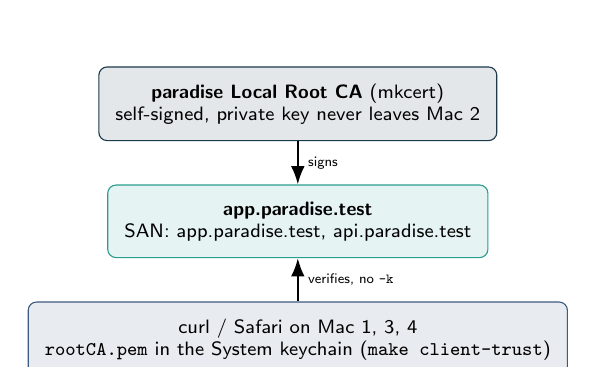
\begin{tikzpicture}[font=\sffamily\scriptsize, node distance=0.55cm]
  \node[draw=lmNavy, fill=lmNavy!12, rounded corners=3pt, align=center, inner sep=6pt] (ca)
    {\textbf{paradise Local Root CA} (mkcert)\\self-signed, private key never leaves Mac 2};
  \node[draw=lmTeal, fill=lmTeal!12, rounded corners=3pt, align=center, inner sep=6pt, below=of ca] (srv)
    {\textbf{app.paradise.test}\\SAN: app.paradise.test, api.paradise.test};
  \node[draw=lmBlue, fill=lmBlue!12, rounded corners=3pt, align=center, inner sep=6pt, below=of srv] (cli)
    {curl / Safari on Mac 1, 3, 4\\\texttt{rootCA.pem} in the System keychain (\texttt{make client-trust})};
  \draw[-{Latex}, thick] (ca) -- node[right, font=\tiny] {signs} (srv);
  \draw[-{Latex}, thick] (cli) -- node[right, font=\tiny] {verifies, no \texttt{-k}} (srv);
\end{tikzpicture}%
}

% ---------- Phase 1: OSI mapping ----------
\newcommand{\drawOsi}{%
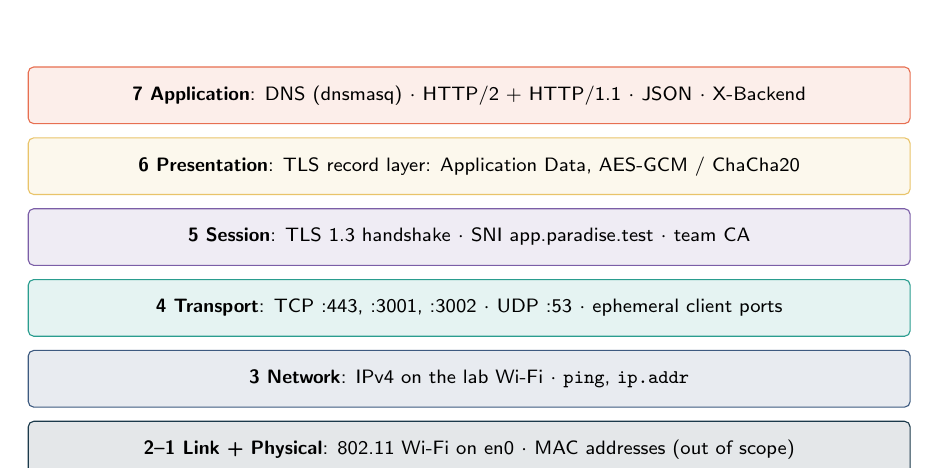
\begin{tikzpicture}[font=\sffamily\scriptsize]
  \foreach \y/\c/\t/\n in {
    5.1/lmCoral/7 Application/{DNS (dnsmasq) $\cdot$ HTTP/2 + HTTP/1.1 $\cdot$ JSON $\cdot$ X-Backend},
    4.2/lmSand/6 Presentation/{TLS record layer: Application Data, AES-GCM / ChaCha20},
    3.3/lmPurple/5 Session/{TLS 1.3 handshake $\cdot$ SNI app.paradise.test $\cdot$ team CA},
    2.4/lmTeal/4 Transport/{TCP :443, :3001, :3002 $\cdot$ UDP :53 $\cdot$ ephemeral client ports},
    1.5/lmBlue/3 Network/{IPv4 on the lab Wi-Fi $\cdot$ \texttt{ping}, \texttt{ip.addr}},
    0.6/lmNavy/2--1 Link + Physical/{802.11 Wi-Fi on en0 $\cdot$ MAC addresses (out of scope)}
  } {
    \node[draw=\c, fill=\c!12, rounded corners=2pt, minimum width=11.2cm,
          minimum height=0.72cm, anchor=west] at (0,\y) {\textbf{\t}: \n};
  }
\end{tikzpicture}%
}

% ---------- Phase 1 + 2: top-down diagnosis ladder ----------
\newcommand{\drawDiagnose}{%
\begin{tikzpicture}[font=\sffamily\scriptsize, node distance=0.22cm]
  \tikzset{st/.style={draw=##1, fill=##1!12, rounded corners=2pt, align=left,
           inner sep=4pt, text width=5.1cm, minimum height=0.62cm, anchor=west, line width=0.7pt},
           ff/.style={font=\sffamily\tiny, align=left, anchor=west, text=lmInk}}
  \node[st=lmNavy]   (l0) at (0,0)     {\textbf{0 Local config}\quad resolvers, /etc/hosts};
  \node[st=lmCoral]  (l1) at (0,-0.85) {\textbf{1 DNS}\quad \texttt{dig @primary}, \texttt{@backup}};
  \node[st=lmBlue]   (l2) at (0,-1.7)  {\textbf{2 Network}\quad \texttt{ping <ip>}};
  \node[st=lmTeal]   (l3) at (0,-2.55) {\textbf{3 Transport}\quad TCP connect :443};
  \node[st=lmPurple] (l4) at (0,-3.4)  {\textbf{4 TLS}\quad \texttt{curl -v} without \texttt{-k}};
  \node[st=lmSand]   (l5) at (0,-4.25) {\textbf{5 HTTP}\quad \texttt{curl -i}};
  \foreach \a/\b in {l0/l1,l1/l2,l2/l3,l3/l4,l4/l5}
    \draw[-{Latex}, thick, lmInk] (\a.south west) ++(0.35,0) -- ++(0,-0.23);
  \node[ff] at (5.7,0)     {wrong resolver $\Rightarrow$ the client never asks Mac 1};
  \node[ff] at (5.7,-0.85) {NXDOMAIN / timeout / an IP that is not an edge};
  \node[ff] at (5.7,-1.7)  {host unreachable (a sleeping Mac may still reply)};
  \node[ff] at (5.7,-2.55) {\textbf{refused} = no listener (RST) $\cdot$ \textbf{timeout} = dropped};
  \node[ff] at (5.7,-3.4)  {curl 60 = CA not trusted $\cdot$ curl 35 = handshake failure};
  \node[ff] at (5.7,-4.25) {502 / 504 = edge up, backends not};
  \draw[lmRed, thick, -{Latex}] (-0.45,0.2) -- node[left, rotate=90, anchor=south, font=\sffamily\tiny, text=lmRed] {stop at the first failure} (-0.45,-4.45);
\end{tikzpicture}%
}

% ---------- Phase 2: keep-alive timer race (Incident 2) ----------
\newcommand{\drawKeepalive}{%
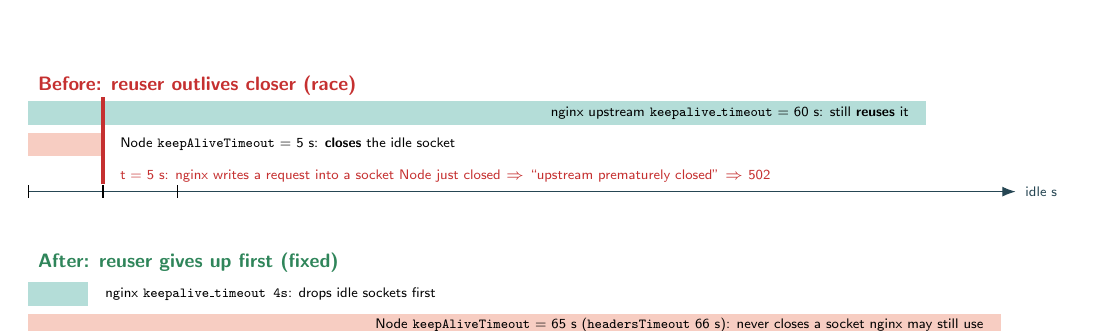
\begin{tikzpicture}[font=\sffamily\scriptsize, x=0.95cm]
  % before
  \node[anchor=west, font=\sffamily\bfseries\scriptsize, text=lmRed] at (0,2.55) {Before: reuser outlives closer (race)};
  \draw[lmInk, -{Latex}] (0,1.2) -- (13.2,1.2) node[right, font=\tiny] {idle s};
  \foreach \x in {0,5,10} \draw (\x*0.2,1.12) -- (\x*0.2,1.28);
  \fill[lmCoral!35] (0,1.65) rectangle (1.0,1.95);
  \node[anchor=west, font=\tiny] at (1.1,1.8) {Node \texttt{keepAliveTimeout} = 5 s: \textbf{closes} the idle socket};
  \fill[lmTeal!35] (0,2.05) rectangle (12,2.35);
  \node[anchor=east, font=\tiny] at (11.9,2.2) {nginx upstream \texttt{keepalive\_timeout} = 60 s: still \textbf{reuses} it};
  \draw[lmRed, very thick] (1.0,1.3) -- (1.0,2.4);
  \node[font=\tiny, text=lmRed, align=left, anchor=west] at (1.1,1.4) {t = 5 s: nginx writes a request into a socket Node just closed $\Rightarrow$ ``upstream prematurely closed'' $\Rightarrow$ 502};
  % after
  \node[anchor=west, font=\sffamily\bfseries\scriptsize, text=lmGreen] at (0,0.3) {After: reuser gives up first (fixed)};
  \fill[lmTeal!35] (0,-0.25) rectangle (0.8,0.05);
  \node[anchor=west, font=\tiny] at (0.9,-0.1) {nginx \texttt{keepalive\_timeout 4s}: drops idle sockets first};
  \fill[lmCoral!35] (0,-0.65) rectangle (13.0,-0.35);
  \node[anchor=east, font=\tiny] at (12.9,-0.5) {Node \texttt{keepAliveTimeout} = 65 s (\texttt{headersTimeout} 66 s): never closes a socket nginx may still use};
\end{tikzpicture}%
}

% ---------- Phase 2: CLOSED vs FILTERED ----------
\newcommand{\drawFiltered}{%
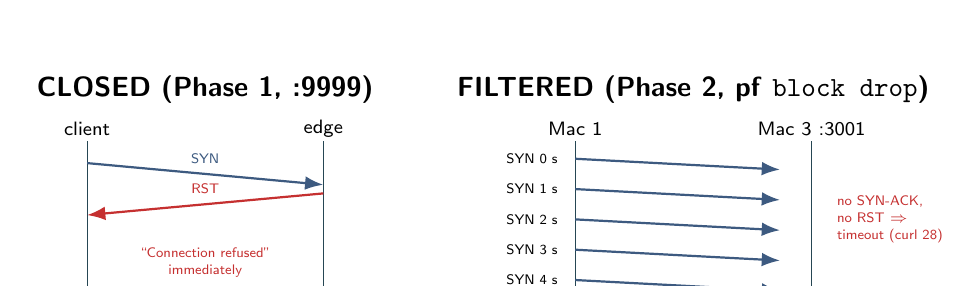
\begin{tikzpicture}[font=\sffamily\scriptsize, y=0.55cm]
  \node[font=\bfseries] at (1.5,6.2) {CLOSED (Phase 1, :9999)};
  \node at (0,5.3) {client}; \node at (3,5.3) {edge};
  \draw[lmInk] (0,5) -- (0,1.5); \draw[lmInk] (3,5) -- (3,1.5);
  \draw[-{Latex}, thick, lmBlue] (0,4.5) -- node[above, font=\tiny] {SYN} (3,4.0);
  \draw[-{Latex}, thick, lmRed] (3,3.8) -- node[above, font=\tiny] {RST} (0,3.3);
  \node[font=\tiny, align=center, text=lmRed] at (1.5,2.2) {``Connection refused''\\immediately};
  \begin{scope}[xshift=6.2cm]
  \node[font=\bfseries] at (1.5,6.2) {FILTERED (Phase 2, pf \texttt{block drop})};
  \node at (0,5.3) {Mac 1}; \node at (3,5.3) {Mac 3 :3001};
  \draw[lmInk] (0,5) -- (0,1.5); \draw[lmInk] (3,5) -- (3,1.5);
  \foreach \y/\t in {4.6/0 s,3.9/1 s,3.2/2 s,2.5/3 s,1.8/4 s}
    { \draw[-{Latex}, thick, lmBlue] (0,\y) -- (2.6,\y-0.25); \node[font=\tiny, anchor=east] at (-0.1,\y) {SYN \t}; }
  \node[font=\tiny, align=left, anchor=west, text=lmRed] at (3.2,3.2) {no SYN-ACK,\\no RST $\Rightarrow$\\timeout (curl 28)};
  \end{scope}
\end{tikzpicture}%
}


\hypersetup{
  colorlinks=true,
  linkcolor=lmNavy,
  urlcolor=lmTeal,
  pdftitle={paradise Project Report},
  pdfauthor={Nipun, Anushka, Tajuddin Shaik, Omkar Hadole}
}
\graphicspath{{figures/}}
\captionsetup{font=small,labelfont=bf}

\titleformat{\section}{\Large\bfseries\color{lmNavy}}{\thesection}{0.6em}{}
\titleformat{\subsection}{\large\bfseries\color{lmTeal}}{\thesubsection}{0.5em}{}
\titleformat{\subsubsection}{\normalsize\bfseries\color{lmInk}}{\thesubsubsection}{0.4em}{}

\pagestyle{fancy}
\fancyhf{}
\fancyhead[L]{\small paradise --- Project report}
\fancyhead[R]{\small Computer Networks (CSA223)}
\fancyfoot[C]{\thepage}
\renewcommand{\headrulewidth}{0.4pt}
\setlength{\headheight}{14pt}

\lstset{
  basicstyle=\ttfamily\footnotesize,
  frame=single,
  rulecolor=\color{lmNavy!30},
  backgroundcolor=\color{lmNavy!4},
  breaklines=true,
  columns=fullflexible,
  keepspaces=true
}

\setlist{itemsep=3pt, topsep=4pt}
\setstretch{1.12}
\setlength{\emergencystretch}{3em}
\newcolumntype{L}[1]{>{\raggedright\arraybackslash}p{#1}}
\sloppy
\widowpenalty=10000
\clubpenalty=10000
\brokenpenalty=10000
\newcommand{\pass}{\textcolor{lmGreen}{\textbf{PASS}}}
\newcommand{\ok}{\textcolor{lmGreen}{\checkmark}}
\newcommand{\bad}{\textcolor{lmRed}{$\times$}}


% Float placement: fill pages, avoid half-empty pages
\renewcommand{\topfraction}{0.9}
\renewcommand{\bottomfraction}{0.8}
\renewcommand{\textfraction}{0.07}
\renewcommand{\floatpagefraction}{0.75}
\setcounter{topnumber}{3}
\setcounter{totalnumber}{4}
\setlength{\textfloatsep}{14pt plus 4pt minus 2pt}
\setlength{\floatsep}{12pt plus 3pt minus 2pt}
\captionsetup[table]{skip=6pt}

% Table of contents
\renewcommand{\cftsecfont}{\bfseries\color{lmNavy}}
\renewcommand{\cftsecpagefont}{\bfseries\color{lmNavy}}
\setlength{\cftsecnumwidth}{2.2em}
\setlength{\cftsubsecindent}{2.2em}
\setlength{\cftsubsecnumwidth}{3.0em}
\setlength{\cftbeforesecskip}{5pt}
\renewcommand{\cftpartfont}{\large\bfseries\color{lmTeal}}
\renewcommand{\cftpartpagefont}{\large\bfseries\color{lmTeal}}
\renewcommand{\cftpartpresnum}{Part~}
\setlength{\cftpartnumwidth}{4.2em}
\setlength{\cftbeforepartskip}{16pt}
\renewcommand{\cfttoctitlefont}{\Huge\bfseries\color{lmNavy}}
\renewcommand{\cftaftertoctitle}{\par\vspace{-6pt}{\color{lmTeal}\rule{\textwidth}{1.2pt}}}

% Parts: one per phase, each on a new page
\renewcommand{\thepart}{\arabic{part}}
\titleformat{name=\part,numberless}[display]{\bfseries\color{lmNavy}\raggedright\hyphenpenalty=10000}{}{0pt}{\LARGE}[{\color{lmTeal}\titlerule[1.6pt]}]
\titlespacing*{\part}{0pt}{0pt}{18pt}

\begin{document}

\begin{titlepage}
\pagecolor{lmNavy}
\color{white}
\setlength{\parindent}{0pt}
\vspace*{0.4cm}
{\small\color{lmTeal}\textbf{COMPUTER NETWORKS (CSA223) \quad$\cdot$\quad PROJECT REPORT}}\par
\vspace{3.2cm}
{\fontsize{46}{50}\selectfont\bfseries paradise}\par
\vspace{10pt}
{\LARGE Private Network Service Platform}\par
\vspace{18pt}
{\color{lmTeal}\rule{5cm}{3pt}}\par
\vspace{18pt}
{\large Phase 1 \;--\; Build and observe the network}\par
\vspace{4pt}
{\large Phase 2 \;--\; Harden, recover and troubleshoot}\par
\vspace{2.6cm}
{\small\color{lmTeal}\textbf{TEAM PARADISE}}\par
\vspace{8pt}
{\renewcommand{\arraystretch}{1.45}
\begin{tabular}{@{}l@{\hspace{1.4cm}}l@{\hspace{1.4cm}}l@{}}
\color{lmTeal}\footnotesize NAME & \color{lmTeal}\footnotesize ENROLMENT & \color{lmTeal}\footnotesize MACHINE AND ROLE \\
Nipun & 2401010323 & Mac 1 $\cdot$ private DNS \\
Anushka & 2401010090 & Mac 2 $\cdot$ edge: nginx, TLS, load balancing \\
Tajuddin Shaik & 2401010436 & Mac 3 $\cdot$ Backend A, caching, tooling \\
Omkar Hadole & 2401010175 & Mac 4 $\cdot$ Backend B, backup DNS, standby edge \\
\end{tabular}}\par
\vfill
\noindent{\color{lmTeal}\rule{\linewidth}{0.6pt}}\par
\vspace{6pt}
{\small Review 1 (Tasks A--G) \;$\cdot$\; Review 2 (Extensions A--F) \hfill Zone \texttt{paradise.test} \;$\cdot$\; November 2026}\par
\end{titlepage}
\nopagecolor
\color{black}

\tableofcontents
\newpage

\section{Abstract}
paradise is a fully local private service. A client types
\texttt{https://app.paradise.test/api/status}, resolves the name through the team's own DNS,
completes TLS at a reverse proxy, and receives JSON from one of two backend replicas. The four
network roles run on four physical MacBooks on the lab Wi-Fi: Mac~1 runs dnsmasq, Mac~2 runs
nginx (TLS termination and round-robin load balancing), and Macs~3 and~4 run the two Express
backends.

\textbf{Part~1 (Phase~1, Review~1)} builds and observes that system: architecture, protocol
mapping, implementation, packet captures of DNS, TCP and TLS, HTTP caching with a deterministic
\texttt{304}, and four failure demonstrations that each break one layer.
\textbf{Part~2 (Phase~2, Review~2)} hardens it without rebuilding it: a backup DNS resolver, a
visible 30-second TTL with DNS-based edge cutover, firewall isolation of the backends,
high-availability failover, a standby edge, and a layer-by-layer troubleshooting method. All six
extensions were demonstrated live, the acceptance test passed 20/20, and four real incidents were
diagnosed, including a keep-alive race between nginx and Node.js that caused six 502s and was fixed.

Every number quoted in this report is taken from the project's evidence files and packet captures (\texttt{evidence/}).

\subsection*{Key results}
\begin{table}[H]
\centering
{\small\renewcommand{\arraystretch}{1.25}
\begin{tabular}{@{}L{3.4cm}L{11.2cm}@{}}
\toprule
\textbf{Area} & \textbf{Result} \\
\midrule
Private DNS & \texttt{app.paradise.test} resolves only through Mac~1; public DNS returns NXDOMAIN \\
HTTPS edge & TLS~1.3 with a team CA, verified without \texttt{-k}; HTTP/2 to the client \\
Load balancing & Both backends in rotation (\texttt{B A A B A B}); deterministic \texttt{304 Not Modified} \\
Acceptance test & \texttt{make p2-verify}: \textbf{20/20} before and after the Phase~2 demos \\
DNS failover & Same query re-sent to the backup resolver \textbf{1.0~s} after the primary went silent \\
TTL and cutover & TTL 30~s; stale window \textbf{9~s} sampled, \textbf{11.4~s} on the wire, 0~s after a flush \\
Isolation & Backend ports \textbf{FILTERED} from clients, \textbf{OPEN} from the edge \\
HA failover & \textbf{145 requests, 0 errors} while Backend~A was stopped and restarted \\
Troubleshooting & 3 injected faults and 4 real incidents diagnosed layer by layer \\
\bottomrule
\end{tabular}}
\end{table}

\clearpage
\part*{{\large\color{lmTeal}PART 1}\protect\\[6pt]Phase 1 --- Build and observe the network}
\addcontentsline{toc}{part}{Part 1\quad Phase 1 --- Build and observe the network}
\section{Purpose and constraints}
The brief asks for a private environment with no cloud. A client must (i)~use a
\texttt{.test} name, (ii)~resolve it through the team DNS, (iii)~open HTTPS on the team edge
with a certificate it genuinely trusts, (iv)~see both backends through the load balancer,
(v)~receive HTTP caching headers and a \texttt{304 Not Modified}, and (vi)~show the whole path
in packet captures.

We used the full four-machine layout: each role runs on its own Mac, so every hop in the
request is a real LAN hop that can be captured. Addresses come from the lab DHCP server,
so they live in one file (\texttt{.env}) and every configuration file is a template rendered
from it. Subnetting, NAT, DHCP, IPv6, routing and Ethernet framing belong to Weeks~7--12
of the syllabus and are deliberately out of scope.

\section{Architecture}

\subsection{Roles versus hardware}
\begin{table}[H]
\centering
\caption{Mapping from the brief to this team.}
{\small
\begin{tabular}{@{}lllll@{}}
\toprule
\textbf{Brief} & \textbf{Owner} & \textbf{LAN identity} & \textbf{Software} & \textbf{Cloud equivalent} \\
\midrule
Mac 1 DNS + client & Nipun & 10.7.27.161 & dnsmasq :53 & Route 53 private zone \\
Mac 2 edge + TLS + LB & Anushka & 10.7.8.155 & nginx :80/:443 & ALB + ACM certificate \\
Mac 3 Backend A & Tajuddin & 10.7.26.203:3001 & Node.js / Express & EC2 target \\
Mac 4 Backend B + client & Omkar & 10.7.18.17:3002 & Node.js / Express & EC2 target \\
\bottomrule
\end{tabular}}
\end{table}

Both backends run \textbf{one codebase} (\texttt{services/backend/}) started as two instances
that differ only in their identity and port. Real addresses live only in \texttt{.env};
\texttt{make render} regenerates \texttt{dnsmasq.conf} and the nginx site from templates.

\subsection{LAN topology}
\begin{figure}[H]
\centering
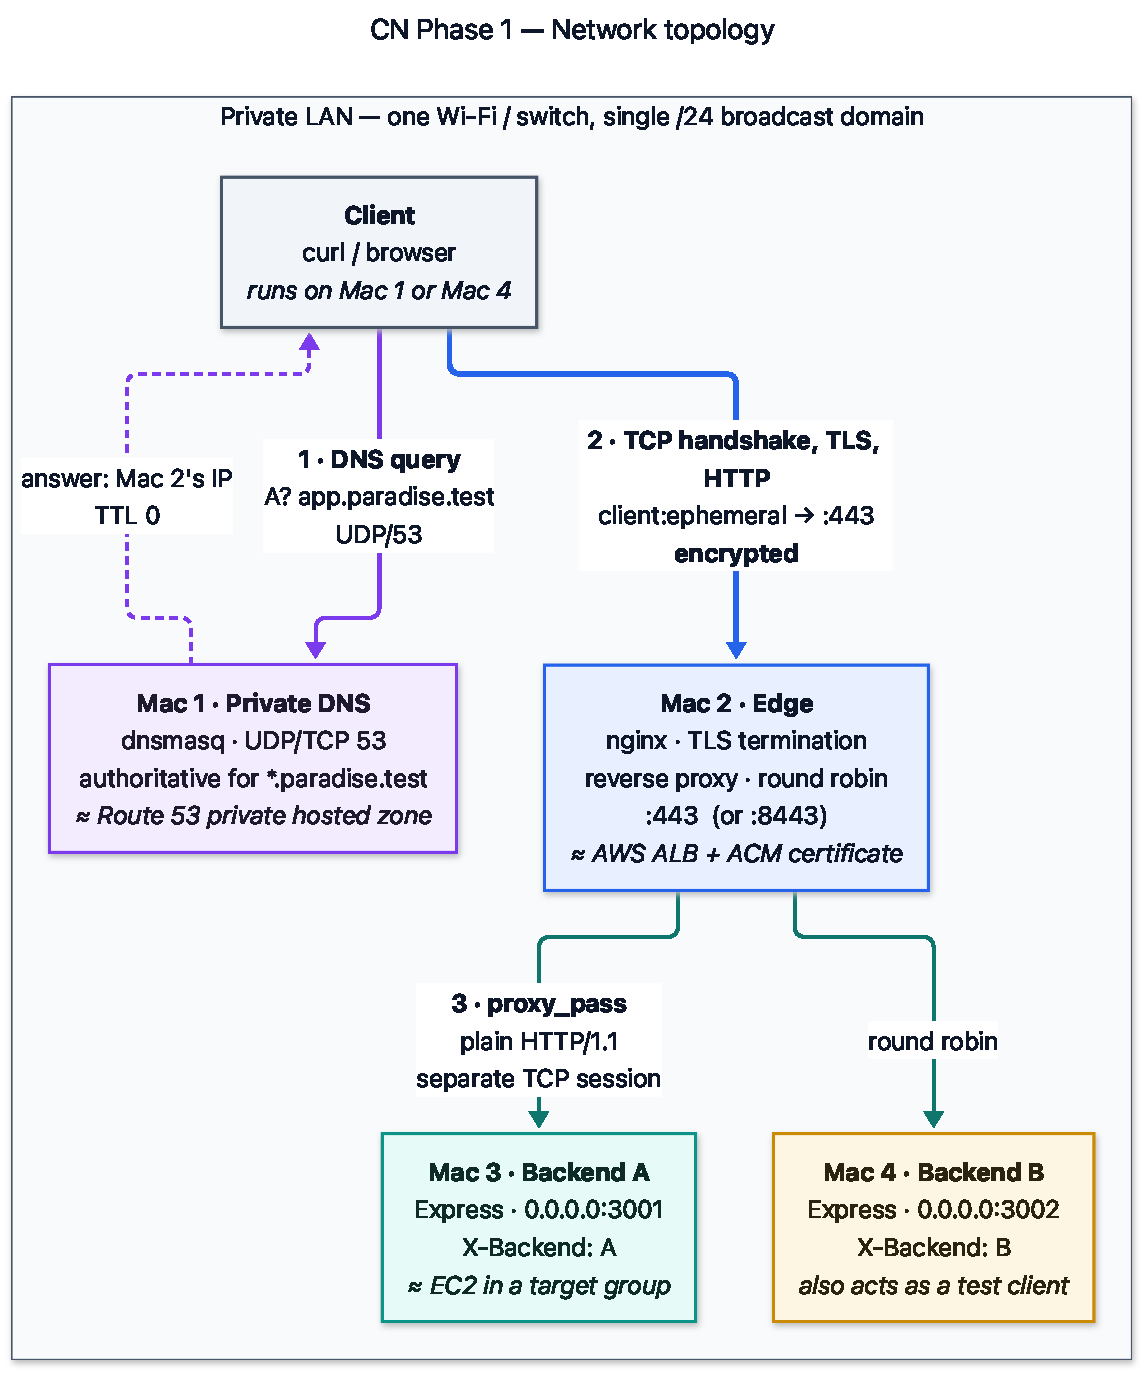
\includegraphics[width=0.74\textwidth]{topology.pdf}
\caption{Phase 1 topology. Clients only ever learn the edge's address from DNS. nginx on
Mac~2 is the only process a client connects to; the backends are reached only by the edge.}
\end{figure}

The structure comes from \emph{which service runs where}, not from the physical network:
all four Macs are on one Wi-Fi network and can reach each other directly. Clients always
use the name; nginx is the only process they treat as ``the service''. The backends could
be renumbered or scaled without any client noticing. That indirection is what a reverse
proxy buys, and it is what makes Phase~2's firewall isolation possible.

\subsection{Request path}
\begin{figure}[H]
\centering
\resizebox{\textwidth}{!}{\drawRequestPath}
\caption{One successful client request, left to right.}
\end{figure}

\begin{figure}[!htbp]
\centering
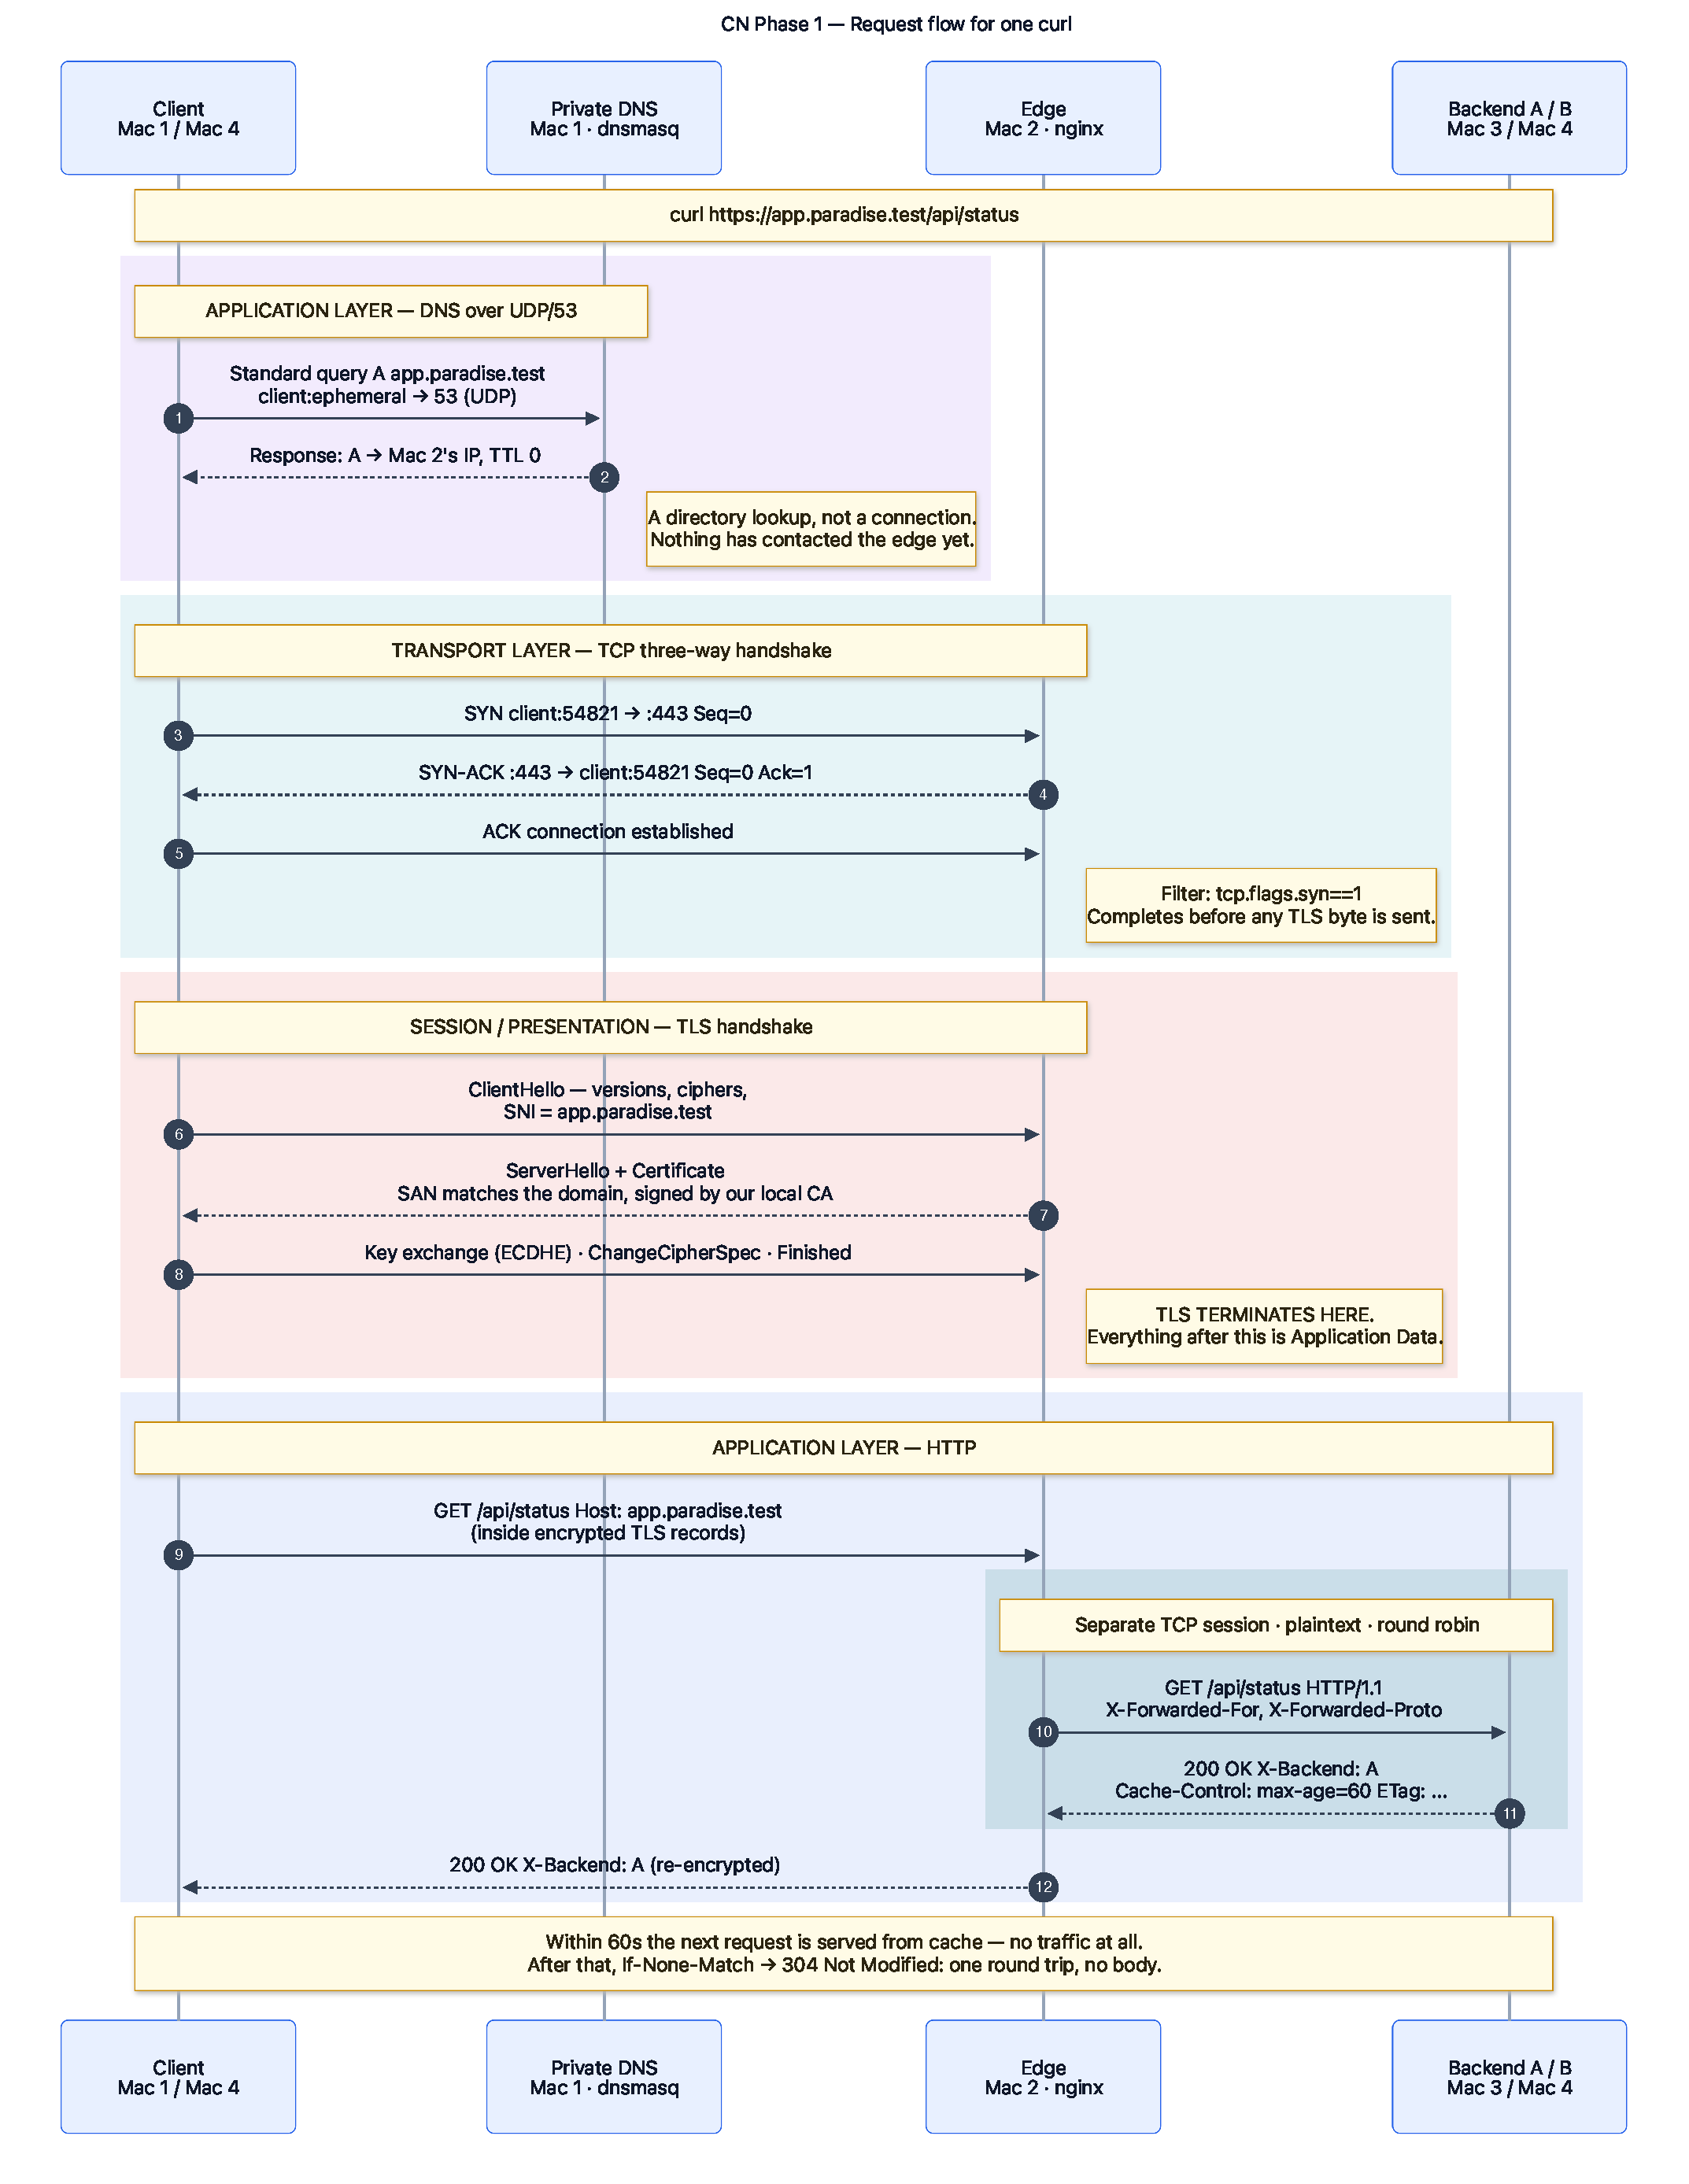
\includegraphics[width=\textwidth,height=0.8\textheight,keepaspectratio]{request-flow.pdf}
\caption{Sequence of one \texttt{curl https://app.paradise.test/api/status}: DNS, TCP, TLS, then
HTTP. nginx opens a separate plaintext connection to the backend it picks.}
\end{figure}

\subsection{Two connections, not one}
\begin{figure}[H]
\centering
\resizebox{\textwidth}{!}{\drawTwoConnections}
\caption{TLS terminates at Mac~2. The client leg and the upstream leg are independent TCP sessions.}
\end{figure}

\begin{table}[!htbp]
\centering
\caption{The two legs of one request.}
{\small
\begin{tabular}{@{}lll@{}}
\toprule
 & \textbf{client $\to$ edge} & \textbf{edge $\to$ backend} \\
\midrule
Protocol & HTTPS (TLS 1.3, HTTP/2 via ALPN) & plain HTTP/1.1 \\
Destination port & 443 & 3001 / 3002 \\
Source port & client ephemeral & nginx ephemeral \\
Readable in Wireshark & no (Application Data) & yes \\
Lifetime & per client connection & pooled and reused (\texttt{keepalive 16}) \\
\bottomrule
\end{tabular}}
\end{table}

\section{Protocol layers}

\begin{figure}[H]
\centering
\drawOsi
\caption{The OSI stack mapped onto paradise. TCP/IP folds layers 5--7 into ``application''.}
\end{figure}

\paragraph{DNS.}
dnsmasq on Mac~1 listens on \texttt{0.0.0.0:53} (UDP and TCP). \texttt{address=/app.paradise.test/}
and \texttt{/api.paradise.test/} answer with the edge's IP; every other name is forwarded
upstream, so clients keep normal internet access. Evidence (A3): from Mac~3,
\texttt{dig app.paradise.test} returns \texttt{status: NOERROR}, flag \texttt{aa}, answer
\texttt{10.7.8.155}, \texttt{SERVER: 10.7.27.161\#53}. The same query to \texttt{@8.8.8.8} returns
\texttt{NXDOMAIN} (A4), which proves the name is genuinely private.
DNS uses UDP because a query fits in one datagram and a lost one is simply retried; a handshake
would double resolution latency.

\paragraph{TCP.}
After resolution the client opens \texttt{10.7.8.155:443} from an ephemeral port:
SYN, SYN-ACK, ACK, before any TLS byte is sent. A connection is identified by its 4-tuple,
so many clients share \texttt{:443} on the edge --- transport-layer demultiplexing.

\paragraph{TLS.}
\begin{figure}[!htbp]
\centering
\drawTls
\caption{Private CA. Clients trust the CA, not the leaf certificate, and never use \texttt{-k}.}
\end{figure}

Observed (C3 and B1): the ClientHello carries SNI \texttt{app.paradise.test} and offers ALPN
\texttt{h2, http/1.1}; the server selects \textbf{TLS 1.3} with
\texttt{TLS\_CHACHA20\_POLY1305\_SHA256} and \textbf{HTTP/2}. The certificate for
\texttt{app.paradise.test} is issued by the paradise Local Root CA and verifies without \texttt{-k}.
The SAN must match the requested host; a CN-only certificate is rejected by every modern client.

\paragraph{HTTP and caching.}
Backends return JSON plus \texttt{X-Backend}, a weak \texttt{ETag}, \texttt{Date} and
\texttt{Cache-Control:} \texttt{public,} \texttt{max-age=60} (D1). The edge adds \texttt{X-Upstream-Addr} and \texttt{X-Edge}.
A conditional request with \texttt{If-None-Match} returns \texttt{304 Not Modified}.

\paragraph{Load balancing.}
nginx's \texttt{upstream} \texttt{backend\_pool} lists both backends with
\texttt{max\_fails=1} and \texttt{fail\_timeout=10s}; the default algorithm is round robin. Six consecutive requests (B2) returned \texttt{B A A B A B},
all \texttt{HTTP/2 200}. nginx is a layer-7 balancer (it reads \texttt{Host} and the path), the
equivalent of an ALB rather than an NLB.

\section{Implementation (what we built, not a runbook)}

\subsection{Private DNS}
Homebrew dnsmasq on Mac~1, rendered from \texttt{infra/mac1-dns/dnsmasq.conf.template}.
\texttt{.test} is reserved by RFC~6761; \texttt{.local} was avoided because macOS sends it to
mDNS/Bonjour. TTL is 0 in Phase~1 so no client holds a stale answer mid-demo.
\texttt{make client-dns} points every Mac's resolver at Mac~1.

\subsection{Backends}
One Express codebase, two instances (\texttt{make backend-a}, \texttt{make backend-b}). Endpoints:
\texttt{GET /}, \texttt{GET /api/status} (identifies the replica), \texttt{GET /api/cacheable}
(byte-identical on both replicas) and \texttt{GET /healthz}. \texttt{src/config.js}
\textbf{refuses to start on 127.0.0.1}: a loopback-bound backend works locally but is invisible
to nginx, so every proxied request would return 502.

\subsection{Edge}
nginx on Mac~2. Port 80 redirects to 443. \texttt{proxy\_pass http://backend\_pool} with
HTTP/1.1 and pooled keep-alive connections; \texttt{proxy\_next\_upstream} retries a failed
attempt on the other backend. A \texttt{default\_server} returns \texttt{444} for requests by IP,
so ``by name, never by IP'' is enforced by the server, not by discipline.

\subsection{TLS}
\texttt{gen-certs.sh} uses mkcert to create the team root CA and a leaf certificate whose SAN covers
\texttt{app.paradise.test} and \texttt{api.paradise.test}. TLS 1.2 and 1.3 only, ECDHE ciphers,
session tickets off. \texttt{make client-trust} installs \texttt{rootCA.pem} on Mac~1, 3 and 4.

\subsection{Tooling}
\texttt{make smoke} runs the whole stack on one laptop (15 checks, no LAN, no sudo).
\texttt{make verify} is the acceptance test: ping matrix, DNS, NXDOMAIN at 8.8.8.8, TLS without
\texttt{-k}, both backends in rotation, 444 by IP, caching headers and a stable 304.
\texttt{make evidence} writes the form answers into \texttt{evidence/}.

\section{Observations and evidence}
Filed under \texttt{evidence/} (index in \texttt{evidence/README.md}):

\begin{table}[!htbp]
\centering
\caption{Evidence collected on 4 October 2026.}
{\small
\begin{tabular}{@{}L{1.0cm}L{4.2cm}L{9.4cm}@{}}
\toprule
\textbf{ID} & \textbf{File} & \textbf{What it shows} \\
\midrule
A1 & \texttt{A1-ips.txt} & Four roles, four IPs, all on \texttt{en0}. \\
A3 & \texttt{A3-dig-client.txt} & \texttt{app.paradise.test} $\to$ 10.7.8.155, \texttt{SERVER} 10.7.27.161, authoritative. \\
A4 & \texttt{A4-dig-8888.txt} & \texttt{@8.8.8.8} $\to$ NXDOMAIN: the zone is private. \\
A5 & \texttt{A5-ping-matrix.txt} & Every pair of Macs: 4/4 replies, 0\% loss. \\
B1 & \texttt{B1-curl-verbose.txt} & TLS 1.3 handshake, certificate verified, HTTP/2 200, no \texttt{-k}. \\
B2 & \texttt{B2-lb-6x.txt} & Six requests: \texttt{B A A B A B}. \\
C1--C3 & \texttt{C-wireshark/} & DNS query/response, TCP handshake, TLS ClientHello with SNI. \\
D1 & \texttt{D1-headers.txt} & \texttt{Cache-Control}, \texttt{ETag}, \texttt{Date}, \texttt{X-Backend}; 304 on revalidation. \\
D3 & \texttt{D3-failure-demo-*.txt} & Failure demonstrations A, B and C (Section~\ref{sec:fail}). \\
\bottomrule
\end{tabular}}
\end{table}

\begin{figure}[!htbp]
\centering
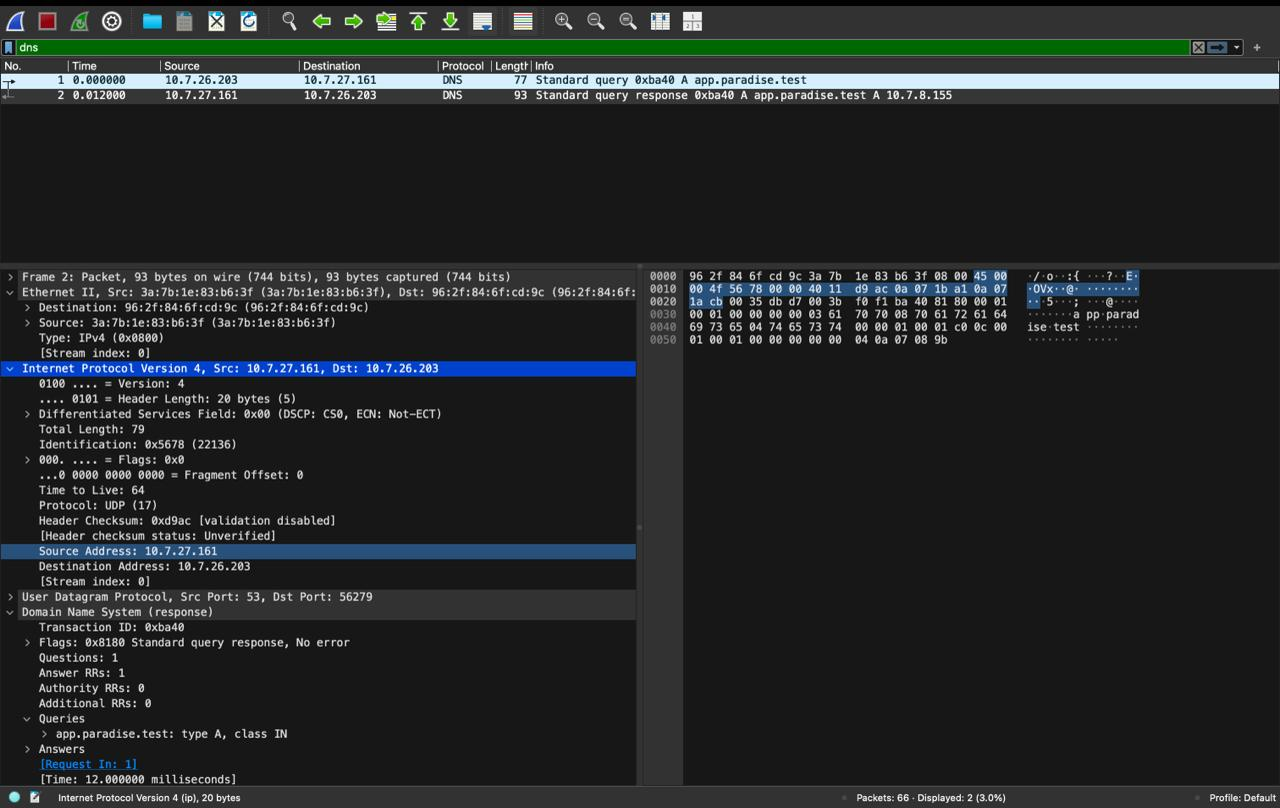
\includegraphics[width=0.88\textwidth]{C1-dns-query-and-response.jpeg}
\caption{C1, filter \texttt{dns}: Mac~3 (10.7.26.203) queries Mac~1 (10.7.27.161) over UDP/53;
the response maps \texttt{app.paradise.test} to 10.7.8.155.}
\end{figure}

\begin{figure}[!htbp]
\centering
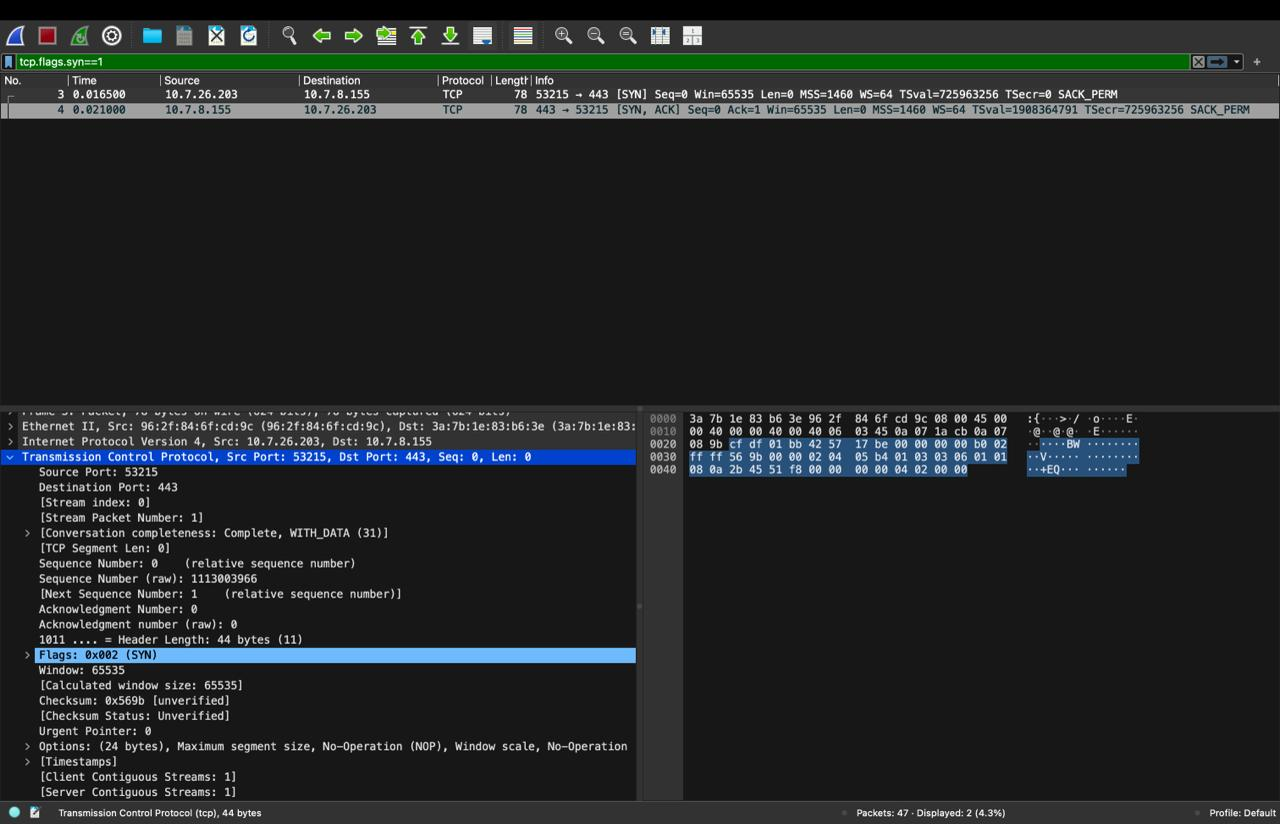
\includegraphics[width=0.88\textwidth]{C2-tcp-syn-and-synack.jpeg}
\caption{C2, filter \texttt{tcp.flags.syn==1}: SYN from an ephemeral port to 10.7.8.155:443 and
the SYN-ACK back, completing before any TLS record.}
\end{figure}

\begin{figure}[!htbp]
\centering
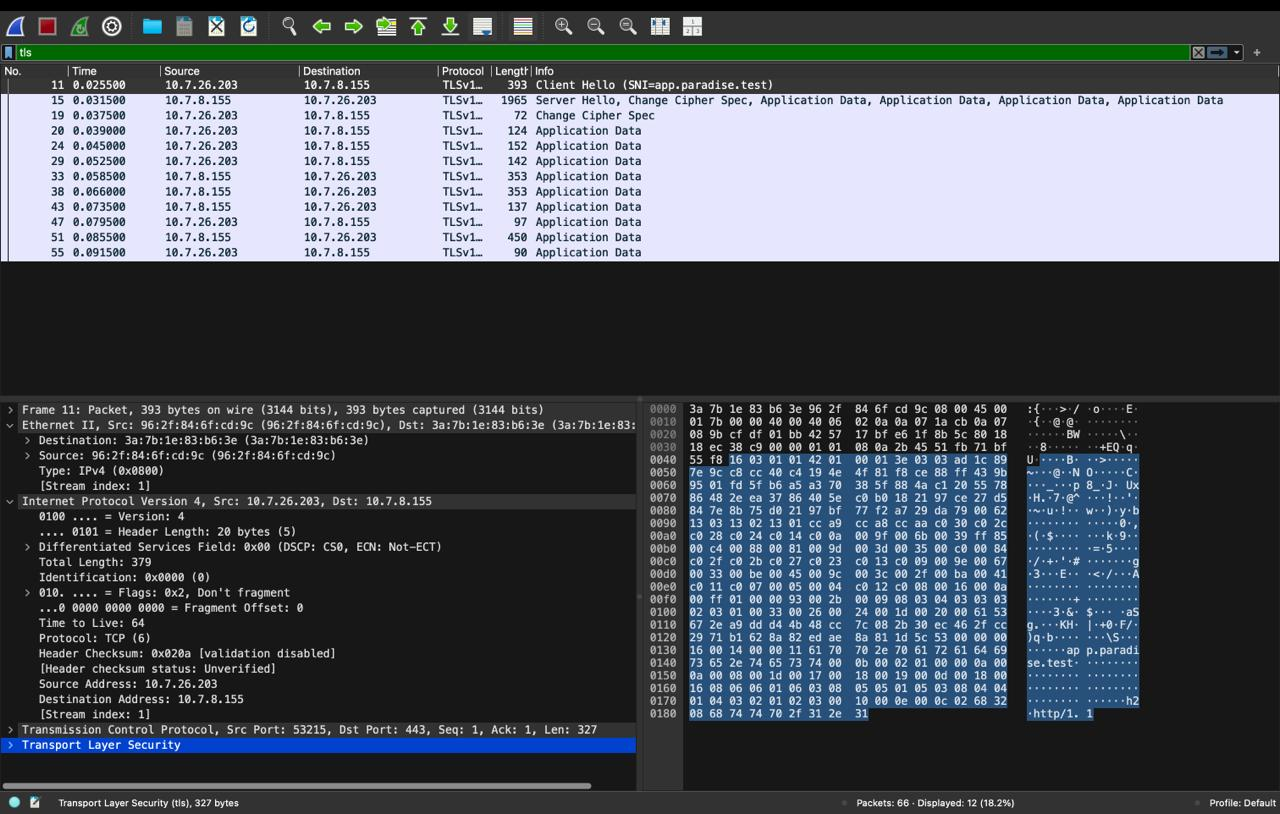
\includegraphics[width=0.88\textwidth]{C3-tls-clienthello-sni.jpeg}
\caption{C3, filter \texttt{tls}: ClientHello with SNI \texttt{app.paradise.test}; everything after the
handshake is opaque Application Data.}
\end{figure}

\paragraph{Why the 304 uses \texttt{/api/cacheable}.}
\texttt{/api/status} must identify its backend, so A and B return different bodies and therefore
different ETags for the same URL. Behind round robin, a conditional request often lands on the
other replica, which does not recognise the validator and returns a full 200: the 304 would
appear only about half the time. \texttt{/api/cacheable} is byte-identical on both machines, so
revalidation is deterministic. \textbf{Validators must agree across replicas, or conditional
requests silently degrade into full responses.}

\section{Failure analysis}\label{sec:fail}
These are the required Phase~1 demonstrations. Each one breaks exactly one layer.

\begin{table}[!htbp]
\centering
\caption{Deliberate faults and the layer they expose (\texttt{make demo-fail}).}
{\small
\begin{tabular}{@{}L{3.0cm}L{5.6cm}L{2.6cm}L{3.2cm}@{}}
\toprule
\textbf{Fault} & \textbf{Observation} & \textbf{Layer} & \textbf{Lesson} \\
\midrule
A: stop Backend A & Before \texttt{BAABAB}; after \texttt{BBBBBB}, all 200; restored \texttt{BAABBA} & application & the edge routes around a dead replica \\
B: client DNS $\to$ 8.8.8.8 & \texttt{dig} NXDOMAIN; \texttt{ping 10.7.8.155} still 0\% loss & application (DNS) & naming and reachability are independent \\
C: request port 9999 & \texttt{Connection refused} after 366 ms; host still pings & transport (TCP) & IP $\neq$ service: RST means no listener \\
D: stop both backends & TLS completes, nginx returns \textbf{502} & application (upstream) & edge is up, origin is not \\
\bottomrule
\end{tabular}}
\end{table}

\begin{figure}[!htbp]
\centering
\resizebox{0.96\textwidth}{!}{\drawDiagnose}
\caption{Diagnosis runs top down; the first step that fails names the layer (\texttt{scripts/status.sh}).}
\end{figure}

\begin{table}[!htbp]
\centering
\caption{Real symptoms met while building, and their causes.}
{\small
\begin{tabular}{@{}L{3.8cm}L{4.8cm}L{5.6cm}@{}}
\toprule
\textbf{Symptom} & \textbf{Cause} & \textbf{Fix} \\
\midrule
\texttt{dig} times out from clients & dnsmasq bound to 127.0.0.1 & \texttt{listen-address=0.0.0.0}, \texttt{make dns} \\
502 on every request & backend bound to loopback & bind \texttt{0.0.0.0}; now refused by \texttt{config.js} \\
\texttt{curl: (60)} & CA not trusted on that Mac & \texttt{make client-trust}, never \texttt{-k} \\
304 only sometimes & testing \texttt{/api/status} & use \texttt{/api/cacheable} \\
\bottomrule
\end{tabular}}
\end{table}

\section{Learning notes (viva)}
\begin{itemize}
  \item DNS finds an IP. TCP then builds a connection. TLS then authenticates the name. HTTP finally carries the request.
  \item DNS is a directory lookup, not a connection: breaking it leaves \texttt{ping} to the IP working.
  \item TLS terminates at the edge. The upstream leg is a separate, plaintext TCP connection.
  \item Trusting \texttt{app.paradise.test.crt} is wrong; trusting the CA is right. The SAN, not the CN, must match.
  \item \texttt{X-Backend} rides back through the proxy untouched, which is what makes round robin visible.
  \item ``Refused'' (RST) and ``timeout'' are different transport-layer answers. Phase~2 uses this distinction.
  \item Mac~2 is the single point of failure: if it dies, DNS still resolves and the backends are healthy, yet nothing is reachable.
\end{itemize}

\clearpage
\part*{{\large\color{lmTeal}PART 2}\protect\\[6pt]Phase 2 --- Harden, recover and troubleshoot}
\addcontentsline{toc}{part}{Part 2\quad Phase 2 --- Harden, recover and troubleshoot}
\section{Phase 2 summary}
Phase~2 hardens the Phase~1 private service without rebuilding it. It adds a backup DNS
resolver, a visible 30-second TTL with DNS-based edge cutover, firewall isolation of the
backends, high-availability failover at the edge, a standby edge, and a layer-by-layer
troubleshooting procedure. All six extensions were demonstrated live on four MacBooks on the
lab Wi-Fi (10.7.0.0/16). Every number below comes from a file in \texttt{evidence/phase2/} or a
capture in \texttt{evidence/captures/}.

\begin{table}[!htbp]
\centering
\caption{Results by extension.}
{\small
\begin{tabular}{@{}L{0.7cm}L{4.3cm}L{1.15cm}L{8.2cm}@{}}
\toprule
\textbf{Ext} & \textbf{Requirement} & \textbf{Result} & \textbf{Key number} \\
\midrule
A & Backup resolver; stop the primary; clients keep resolving & \pass & Same query ID \texttt{0x90b0} re-sent to the backup \textbf{1.0 s} after the primary went silent; \texttt{curl} stayed HTTP 200 \\
B & Visible TTL; old answer until expiry; manual flush & \pass & TTL \textbf{30 s}; stale window \textbf{9 s} sampled, \textbf{11.4 s} on the wire; \textbf{0--2 s} after a flush \\
C & Only the edge reaches :3001/:3002 & \pass & From a client: \textbf{FILTERED} (5 SYNs, no reply). From Mac 2: \textbf{OPEN} \\
D & Kill Backend A under load; zero errors; A rejoins & \pass & \textbf{145 requests, 0 non-200}, 37 consecutive B-only responses, A back at \textbf{50 s} \\
E & DNS cutover to a standby edge; observe the TTL & \pass & \texttt{X-Edge} moved \texttt{nginx@10.7.3.123} $\to$ \texttt{nginx@10.7.18.17}, every request 200 \\
F & Diagnose injected faults layer by layer & \pass & 3 injected faults, 3 correct verdicts, plus 3 real incidents diagnosed the same way \\
--- & Acceptance test \texttt{make p2-verify} & \pass & \textbf{20/20} before the demos (12:11) and after every fault was undone (13:09) \\
\bottomrule
\end{tabular}}
\end{table}

Running the demos for real exposed one design bug: a keep-alive timer race between nginx and
Node.js. Under failover it turned into \textbf{six HTTP 502s}. It was diagnosed from the edge's
error log, fixed with two timer values, and the demo was re-run clean (Section~\ref{sec:inc},
Incident~2). This is the most important thing we learned in Phase~2.

\section{From Phase 1 to Phase 2}
Phase~1 established the path
\texttt{client $\to$ Mac 1 DNS $\to$ Mac 2 nginx/TLS edge $\to$ Backend A (Mac 3) or Backend B (Mac 4)}.
dnsmasq maps the private \texttt{.test} names to the edge; nginx terminates TLS 1.3 on port 443,
balances by round robin to ports 3001 and 3002, and exposes the backend identity through
\texttt{X-Backend}. Phase~1 deliberately left single points of failure: one DNS server, one
edge, backend ports open to the whole LAN, and a TTL of 0 that hid caching entirely.

Phase~2 keeps that topology and asks what happens when a DNS server, a record, a backend, the
edge or a firewall path changes, and proves recovery with observable commands and rollback
material. No new hardware was added: Mac~4 additionally hosts the backup DNS and the standby edge.

\section{Architecture and design decisions}

\begin{figure}[H]
\centering
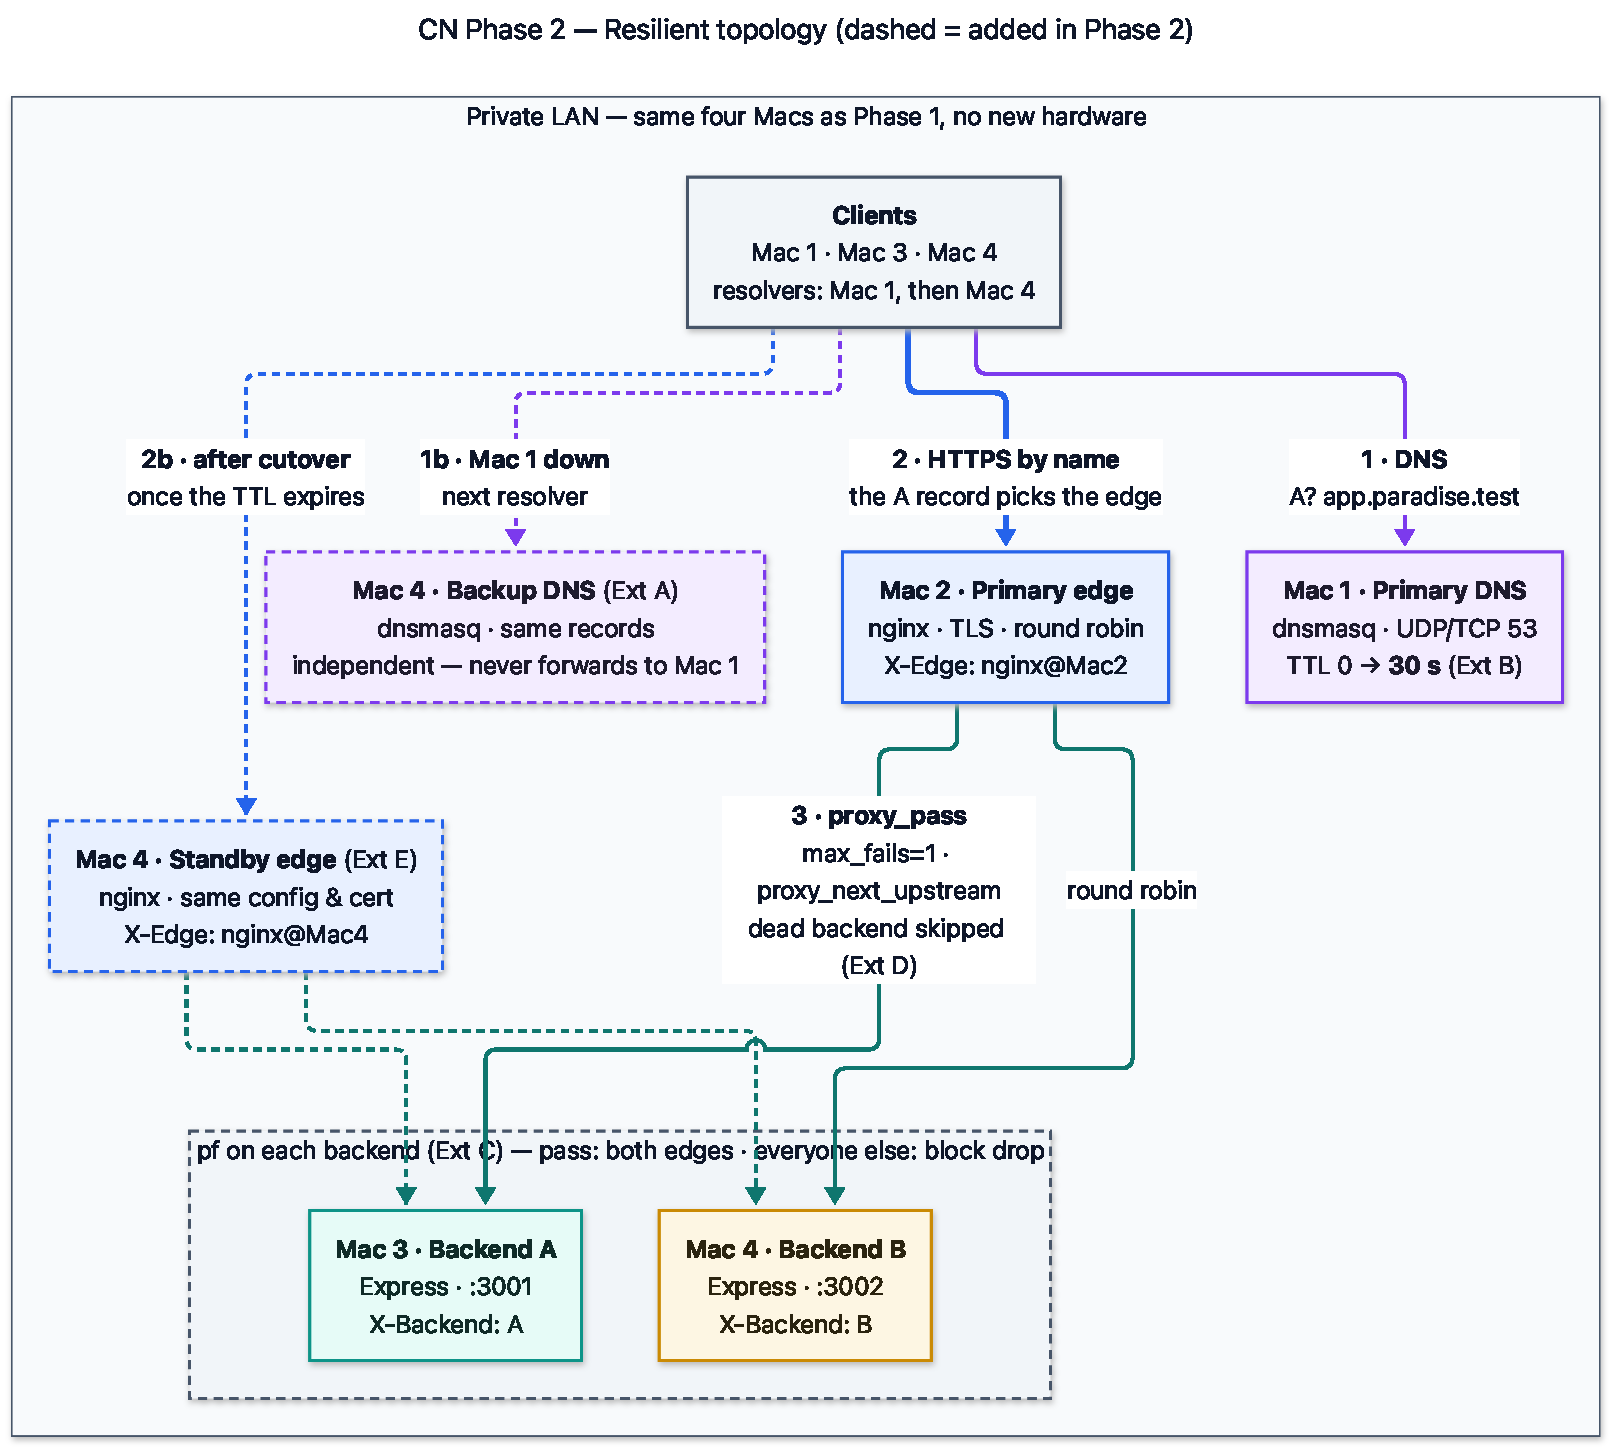
\includegraphics[width=0.85\textwidth]{p2-topology.pdf}
\caption{Topology after Phase~2. Dashed elements were added in Phase~2.}
\end{figure}

\begin{table}[!htbp]
\centering
\caption{What changed from Phase~1, with the cloud equivalent.}
{\small
\begin{tabular}{@{}L{2.7cm}L{3.3cm}L{4.3cm}L{4.0cm}@{}}
\toprule
\textbf{Area} & \textbf{Phase 1} & \textbf{Phase 2} & \textbf{Cloud equivalent} \\
\midrule
DNS servers & one, Mac 1 & two \textbf{independent} servers, Mac 1 + Mac 4 & Route 53's four name servers per zone \\
DNS TTL & 0 s, nothing cached & \textbf{30 s}, caching observable & record TTL lowered before a migration \\
Client resolvers & Mac 1 & Mac 1, \textbf{then} Mac 4 & VPC resolver with fallback \\
Backend ports & reachable by anyone on the LAN & only from the two edges (pf \texttt{block drop}) & Security Group allowing the ALB's SG only \\
Backend failure & passive \texttt{max\_fails} & unchanged, plus a live health view & ALB target health \\
Edge & Mac 2 only & Mac 2 + \textbf{standby on Mac 4}, chosen by DNS & second ALB + Route 53 failover \\
Edge--backend keep-alive & nginx 60 s, Node 5 s (defaults) & nginx \textbf{4 s}, Node \textbf{65 s} & ALB idle timeout $<$ target keep-alive \\
\bottomrule
\end{tabular}}
\end{table}

\paragraph{Backup DNS does not forward to the primary.}
It serves the records itself. A backup that depends on the primary fails together with it. The
cost is that a record change must be applied to both servers (\texttt{make p2-cutover} on each);
in production, zone transfers (AXFR/IXFR) keep secondaries in sync.

\paragraph{pf \texttt{block drop}, not \texttt{block return}.}
A dropped SYN times out (FILTERED); a refused SYN gets a RST (CLOSED). Phase~1's wrong-port demo
already shows CLOSED, so Phase~2's firewall shows a different, distinguishable failure.

\paragraph{pf rules live in an anchor.}
macOS already evaluates \texttt{anchor "com.apple/*"}. We load
\texttt{com.apple/250.ParadiseIsolation} and enable pf with a reference token (\texttt{pfctl -E}).
Rollback flushes that one anchor and releases that one token; no system file is edited.

\paragraph{Health checking stays passive.}
Active \texttt{health\_check} is an nginx Plus feature. Open-source nginx detects failure from real
traffic: \texttt{max\_fails=1 fail\_timeout=10s} marks a dead server down, and
\texttt{proxy\_next\_upstream} retries the same request on the survivor.

\paragraph{The reusing side times out first.}
Not in the original design; found during an Ext~D run (Incident~2). nginx now drops idle upstream
sockets at 4~s and Node keeps them for 65~s.

\paragraph{The standby edge reuses the certificate.}
Clients connect by name, the SAN covers it, and the CA is already trusted on every Mac, so there
is no new trust to distribute.

\section{Implemented repository changes}
Every Phase~2 file lives in a \texttt{phase2/} subfolder of its Phase~1 home:
\begin{itemize}
  \item \texttt{scripts/phase2/}: install, demo, verify, diagnose, fault-injection and rollback scripts, a shared \texttt{lib/p2common.sh}, and \texttt{phase2.mk} (\texttt{make p2} lists every target).
  \item \texttt{infra/phase2/}: the pf isolation template and an optional \texttt{.env.phase2}; rendered configs go to the gitignored \texttt{build/}.
  \item \texttt{docs/phase2/}: runbook, architecture and the final write-up; four new diagrams in \texttt{docs/diagrams/phase2/}.
  \item \texttt{evidence/phase2/}: demo and verification output for A--F, screenshots and a configuration bundle.
\end{itemize}
Phase~2 renders the \emph{same} Phase~1 templates with overrides. \textbf{Phase~1 code changed in
exactly two places}: \texttt{keepalive\_timeout 4s;} in the nginx upstream template and
\texttt{keepAliveTimeout}/\texttt{headersTimeout} in \texttt{services/backend/src/server.js}.
\texttt{make p2-test} asserts those values and fails on any other change to Phase~1 code
(\textbf{55/55} checks pass).

Two tooling fixes were made during the run: \texttt{verify-phase2.sh} now writes every check line
to its evidence file, and \texttt{ha-demo.sh} now requires a B-only window of $\geq$15 consecutive
responses \emph{and} at least one request nginx retried off Backend~A. The old check passed once
when A was never stopped, because round robin produces short B-runs by chance; we caught the false
pass by counting retries (0) and deleted that run.

\section{Verification results}
\texttt{make p2-verify} was run from Mac~1 before the demos (12:11:47) and again after every fault
had been undone (13:09:49). Both runs: \textbf{20 passed, 0 failed}.

\begin{table}[!htbp]
\centering
\caption{Acceptance checks (\texttt{verify-phase2-20261123-130949.txt}).}
{\small
\begin{tabular}{@{}L{0.6cm}L{11.6cm}L{1.4cm}@{}}
\toprule
\textbf{Ext} & \textbf{Check} & \textbf{Status} \\
\midrule
A & client resolvers include primary 10.7.20.228 and backup 10.7.18.17 (2 checks) & \pass \\
A & primary and backup both answer \texttt{app.paradise.test} (2 checks) & \pass \\
A & primary and backup return the same record (10.7.3.123 / 10.7.3.123) & \pass \\
A & backup answers \texttt{api.paradise.test} too; still forwards public names (2 checks) & \pass \\
B & primary and backup serve TTL 30 s (2 checks) & \pass \\
B & record points at a known edge (10.7.3.123) & \pass \\
C & direct 10.7.13.238:3001 and 10.7.18.17:3002 filtered from a client (curl 28) (2 checks) & \pass \\
D & 6 requests \texttt{AABABA}, all 200: A in rotation, B in rotation, no failures (3 checks) & \pass \\
D & primary edge \texttt{/edge-health} = 200 & \pass \\
E & standby edge answers 200, identifies as \texttt{nginx@10.7.18.17}, reaches the backends (3 checks) & \pass \\
F & \texttt{diagnose.sh} present and parses & \pass \\
\midrule
 & \textbf{Total} & \textbf{20/20} \\
\bottomrule
\end{tabular}}
\end{table}

\section{Resilience tests by extension}

\subsection{Extension A --- Backup DNS resolver}
Mac~4 runs a second dnsmasq rendered from the same template. Every client's resolver list is
\texttt{10.7.20.228, 10.7.18.17}. Nipun stopped dnsmasq on Mac~1 (\texttt{make p2-dns-stop}) from
\textbf{12:47:46 to 12:49:43}, observed from three places at once:

\begin{table}[!htbp]
\centering
\caption{Ext~A observed from three vantage points.}
{\small
\begin{tabular}{@{}L{2.4cm}L{8.0cm}L{3.9cm}@{}}
\toprule
\textbf{Vantage point} & \textbf{What it showed} & \textbf{Evidence} \\
\midrule
Mac 3, pure client & \texttt{dig @10.7.20.228} timed out; normal \texttt{dig} $\to$ \texttt{SERVER: 10.7.18.17}, answer 10.7.3.123; \texttt{curl} HTTP 200; afterwards back on the primary & \texttt{A-failover-\allowbreak demo.txt} \\
Mac 1, every 2 s & 0--72 s primary; \textbf{74--189 s} primary DOWN, every lookup still 10.7.3.123 from 10.7.18.17; from 191 s back on the primary & \texttt{A2-failover-\allowbreak watch-mac1.txt} \\
Mac 4 dnsmasq log & Mac 1's queries every $\sim$4 s until 12:49:41, answered \texttt{config} (own data, not forwarded) & \texttt{A3-backup-\allowbreak dnsmasq-log.txt} \\
\bottomrule
\end{tabular}}
\end{table}

\begin{table}[!htbp]
\centering
\caption{Packets in \texttt{p2-A-dns-failover.pcapng}.}
{\small
\begin{tabular}{@{}llL{4.4cm}lL{4.6cm}@{}}
\toprule
\textbf{Frame} & \textbf{Time} & \textbf{Source $\to$ Destination} & \textbf{DNS ID} & \textbf{Meaning} \\
\midrule
228 & 74.35 s & 10.7.20.228 $\to$ 10.7.20.228 & \texttt{0x6933} & query to the primary: no response \\
230 & 75.37 s & 10.7.20.228 $\to$ 10.7.20.228 & \texttt{0x90b0} & next lookup to the primary: no response \\
232 & 76.38 s & 10.7.20.228 $\to$ \textbf{10.7.18.17} & \textbf{\texttt{0x90b0}} & \textbf{the same query} re-sent to the backup, 1.0 s later \\
233 & 76.61 s & 10.7.18.17 $\to$ 10.7.20.228 & \texttt{0x90b0} & \texttt{A 10.7.3.123}, TTL 30 \\
\bottomrule
\end{tabular}}
\end{table}

Over the whole capture the primary answered 117 of 174 queries (57 lost during the outage) and
the backup answered 28 of 28. \textbf{Resolution never stopped}; the cost was a $\sim$1~s resolver
timeout per lookup while the primary was down.

\begin{figure}[!htbp]
\centering
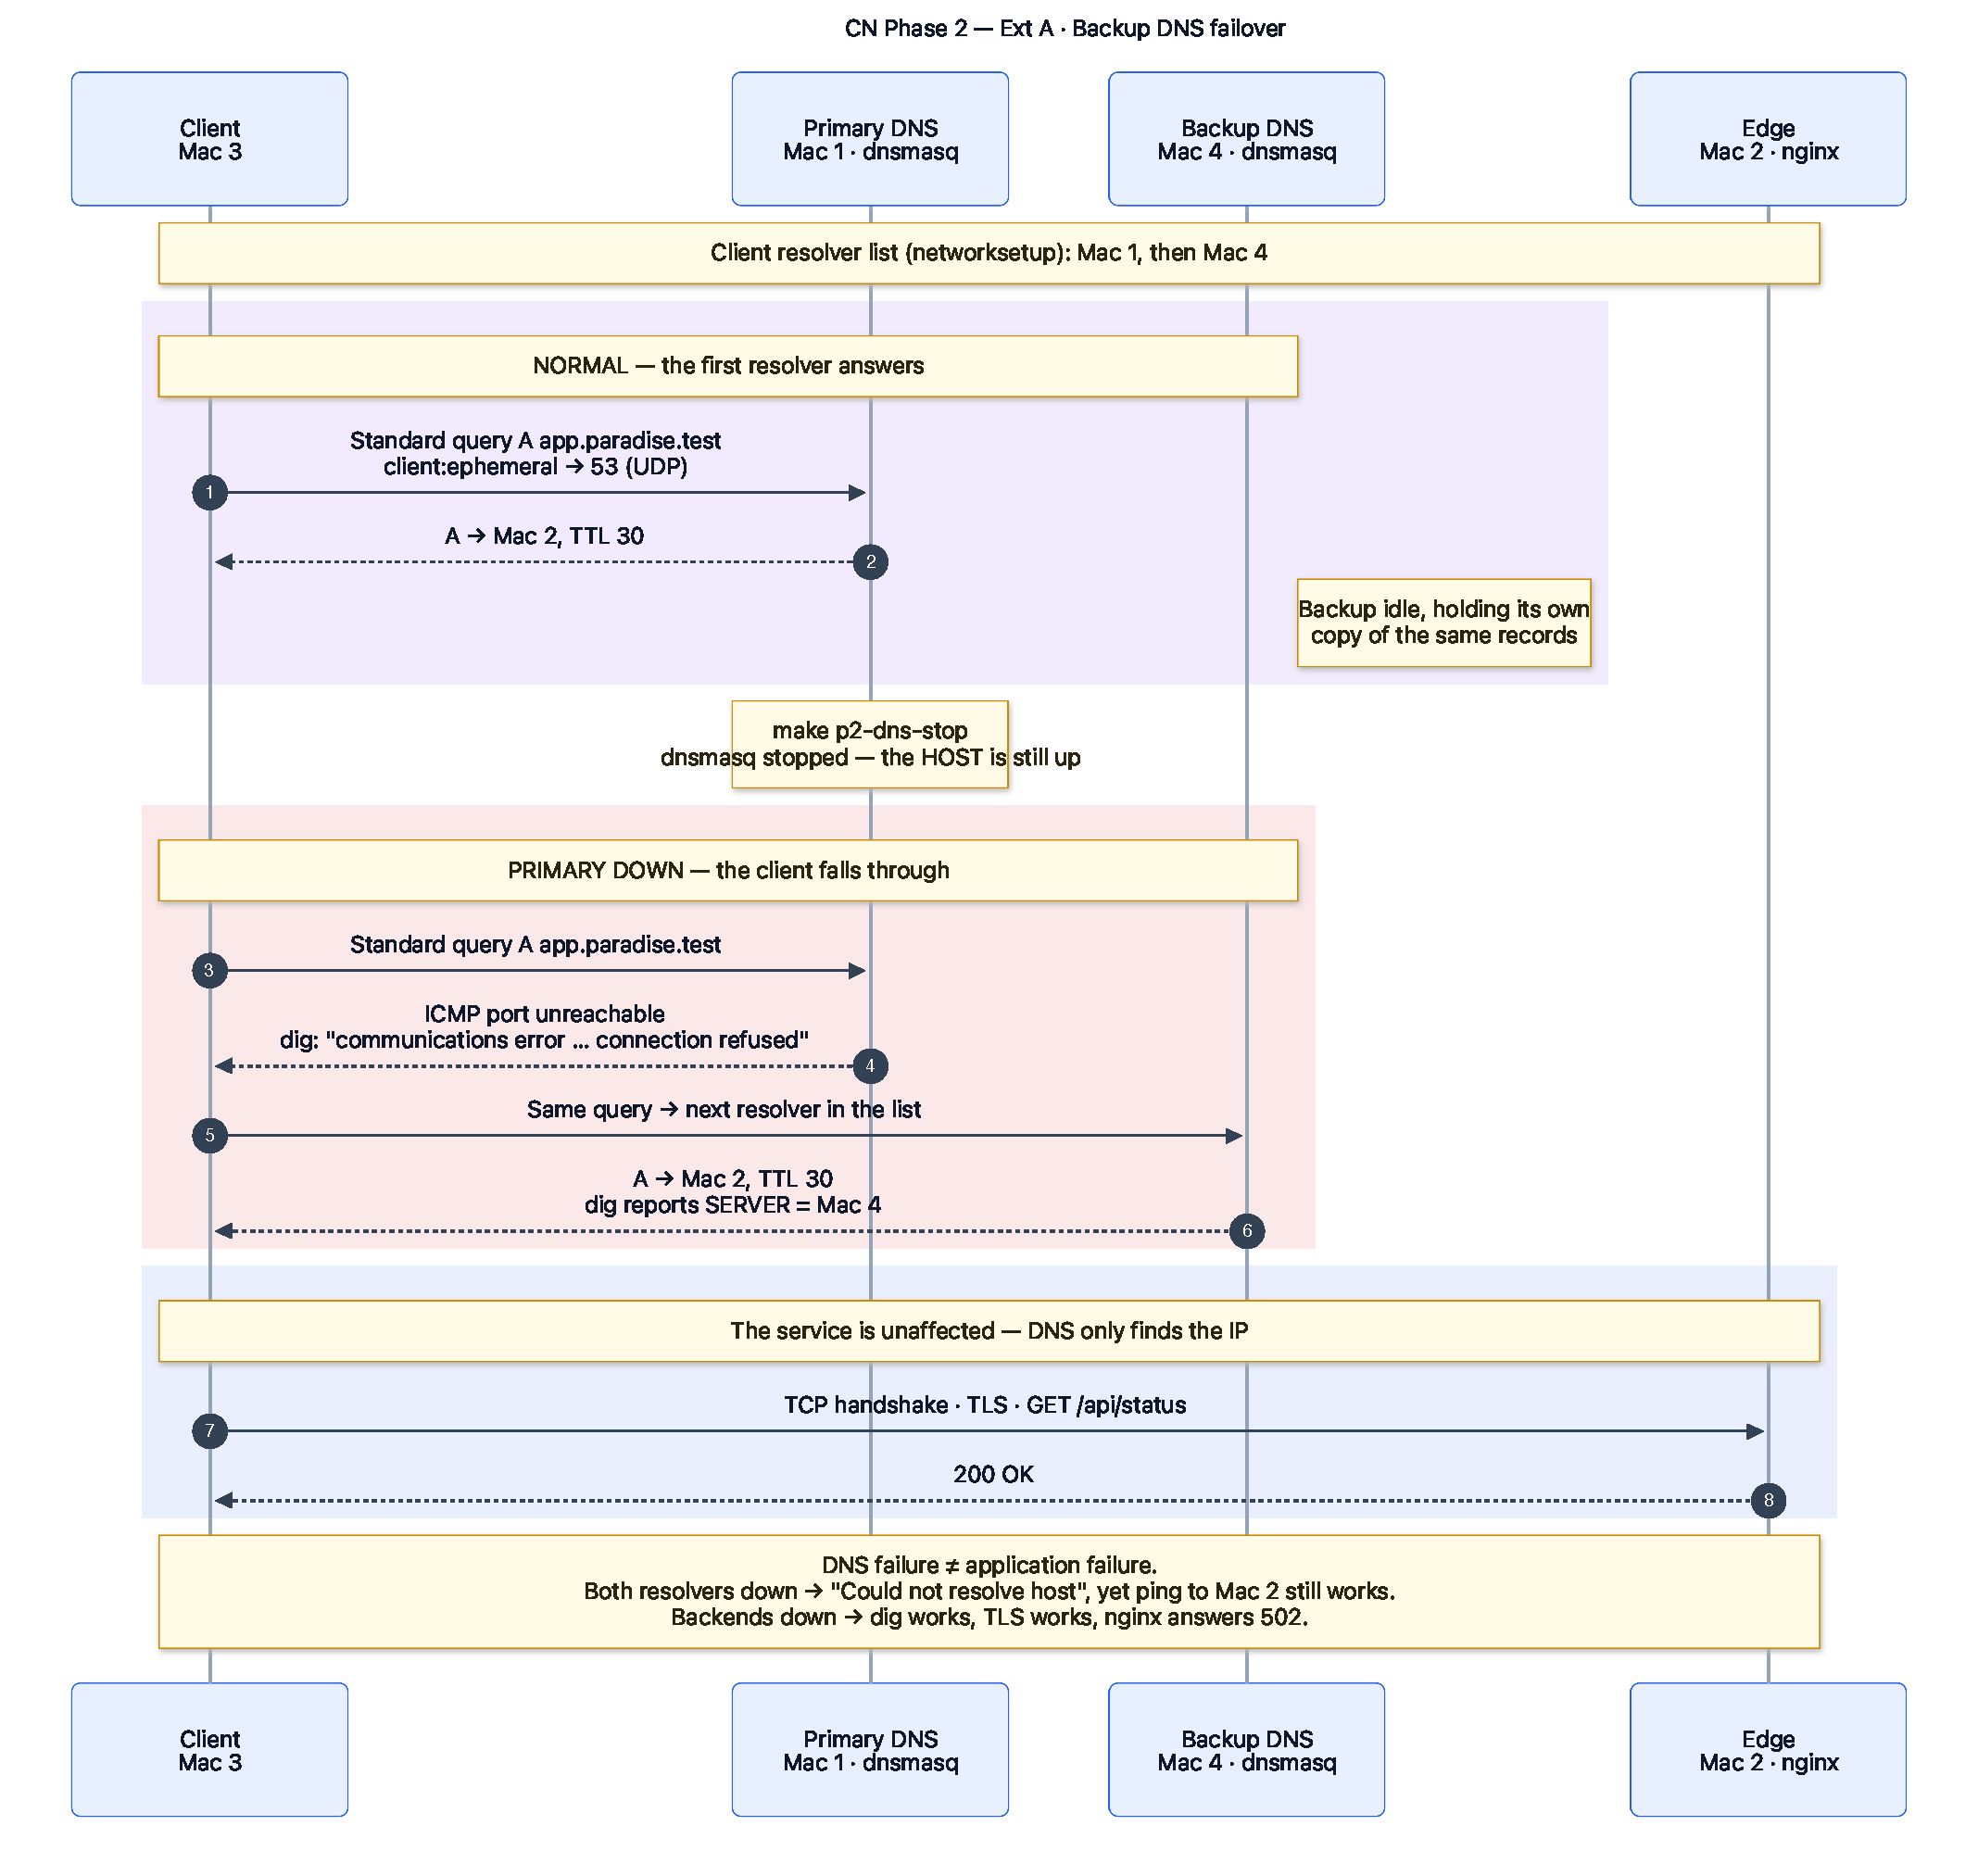
\includegraphics[height=0.62\textheight,keepaspectratio]{p2-dns-failover.pdf}
\caption{Ext~A sequence: the client retries the same query on the next resolver in its list.}
\end{figure}

\begin{figure}[!htbp]
\centering
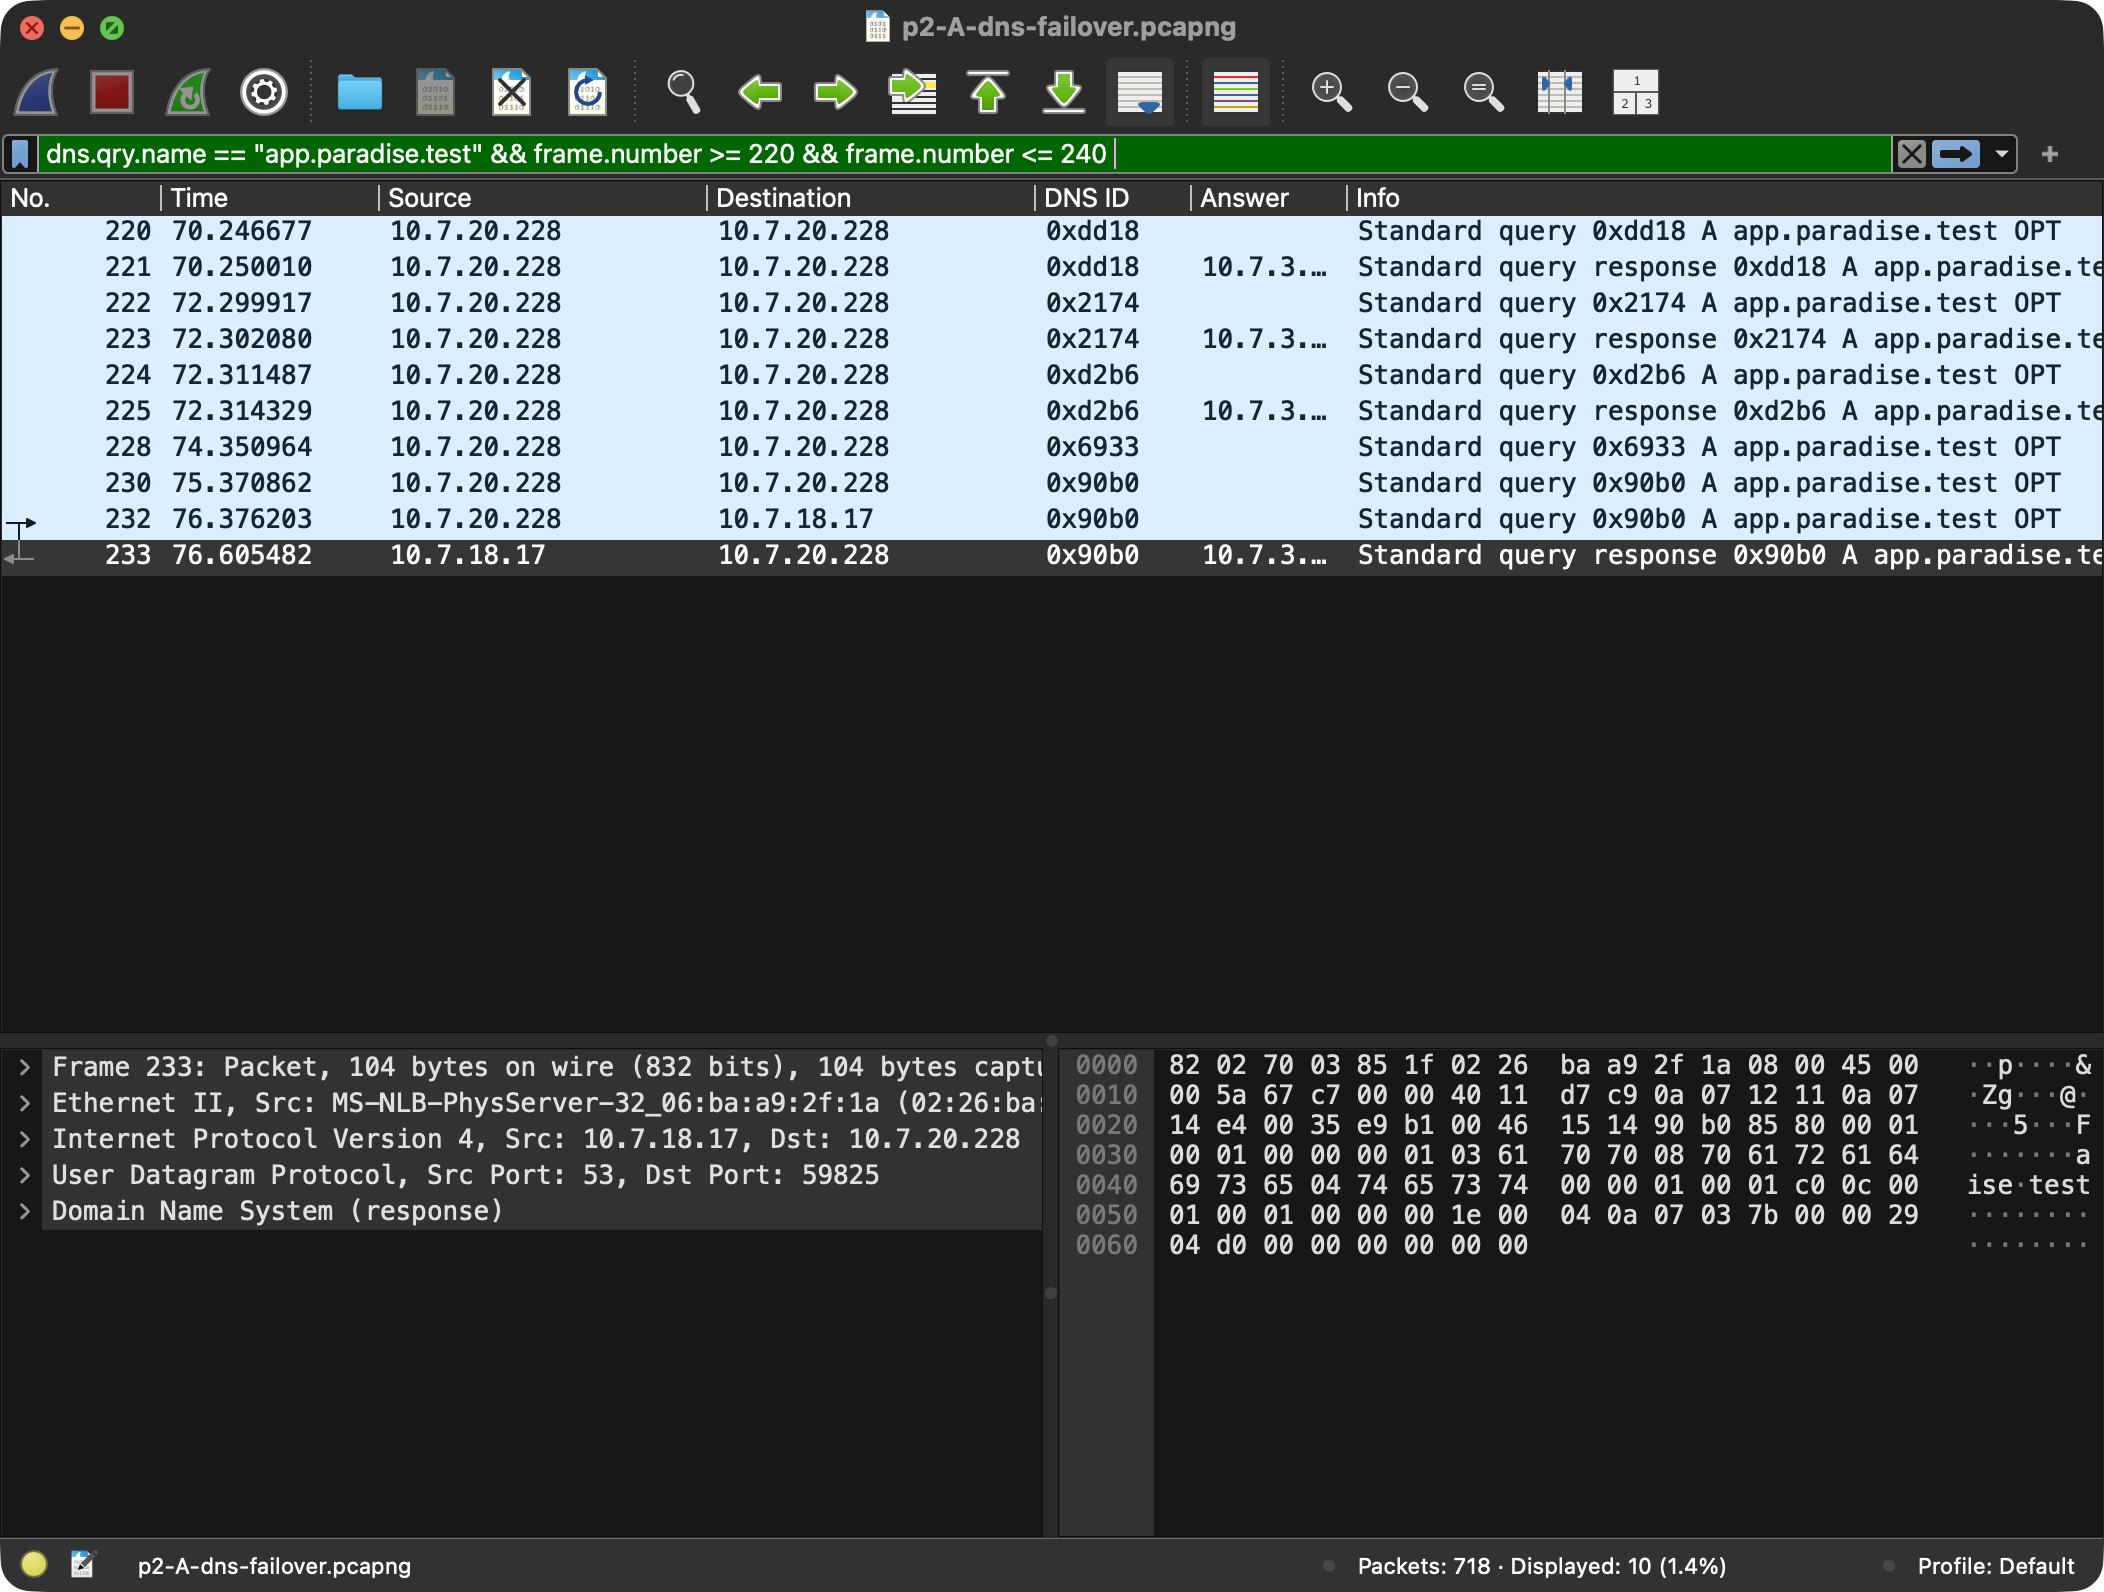
\includegraphics[width=0.85\textwidth]{W-A2-same-id-retried-on-backup.png}
\caption{W-A2: transaction ID \texttt{0x90b0} unanswered by the primary, then re-sent to and answered by the backup 10.7.18.17.}
\end{figure}

\subsection{Extension B --- DNS TTL and controlled record change}
TTL was raised from 0 to \textbf{30 s} on both servers (B1; screenshot W-B1 shows TTL 30 on every
answer). \texttt{make p2-ttl-watch} on Mac~1 printed every $\sim$2~s three different truths side by
side: \texttt{dig} (asks the server, bypasses the cache), the OS cache (what
\texttt{mDNSResponder} hands to applications), and \texttt{curl} (where a real HTTPS request went).
Meanwhile the records were changed with \texttt{make p2-cutover} on Mac~1 and Mac~4.

\begin{table}[!htbp]
\centering
\caption{Stale windows measured by \texttt{p2-ttl-watch}.}
{\small
\begin{tabular}{@{}L{4.9cm}L{1.6cm}L{2.4cm}L{4.8cm}@{}}
\toprule
\textbf{Change} & \textbf{dig flips} & \textbf{cache / curl flip} & \textbf{Stale window} \\
\midrule
primary $\to$ standby (TTL expiry) & 12:55:03 & 12:55:12 & \textbf{9 s} (\texttt{STALE} $\times$4) \\
standby $\to$ primary (TTL expiry) & 12:56:57 & 12:57:06 & \textbf{9 s} (\texttt{STALE} $\times$4) \\
primary $\to$ standby + \texttt{make p2-flush} & 12:59:02 & 12:59:02 & \textbf{0 s} \\
standby $\to$ primary + \texttt{make p2-flush} & 12:59:19 & 12:59:21 & \textbf{2 s} (gap between dnsmasq restart and flush) \\
\bottomrule
\end{tabular}}
\end{table}

\paragraph{On the wire} (\texttt{p2-BE-ttl-cutover.pcapng}): frame \textbf{1002} (65.50 s) is the
first DNS answer carrying 10.7.18.17, yet the TLS ClientHellos in frames 1006, 1040, 1076, 1108 and
1148 still go to 10.7.3.123. The first ClientHello to 10.7.18.17 is frame \textbf{1195} (76.89 s), so
the stale period on the wire was \textbf{11.4 s}. While the cache is valid the OS sends no DNS packet
at all, so staleness is visible only in where TCP connects.

\paragraph{Why 9--11 s and not 30 s.} The TTL counts down from when the OS \emph{fetched} the answer,
not from when the record changed. The cached entry was already $\sim$20~s old at the moment of the
change. Across many clients the stale period is spread uniformly between 0 and 30~s.

\begin{figure}[!htbp]
\centering
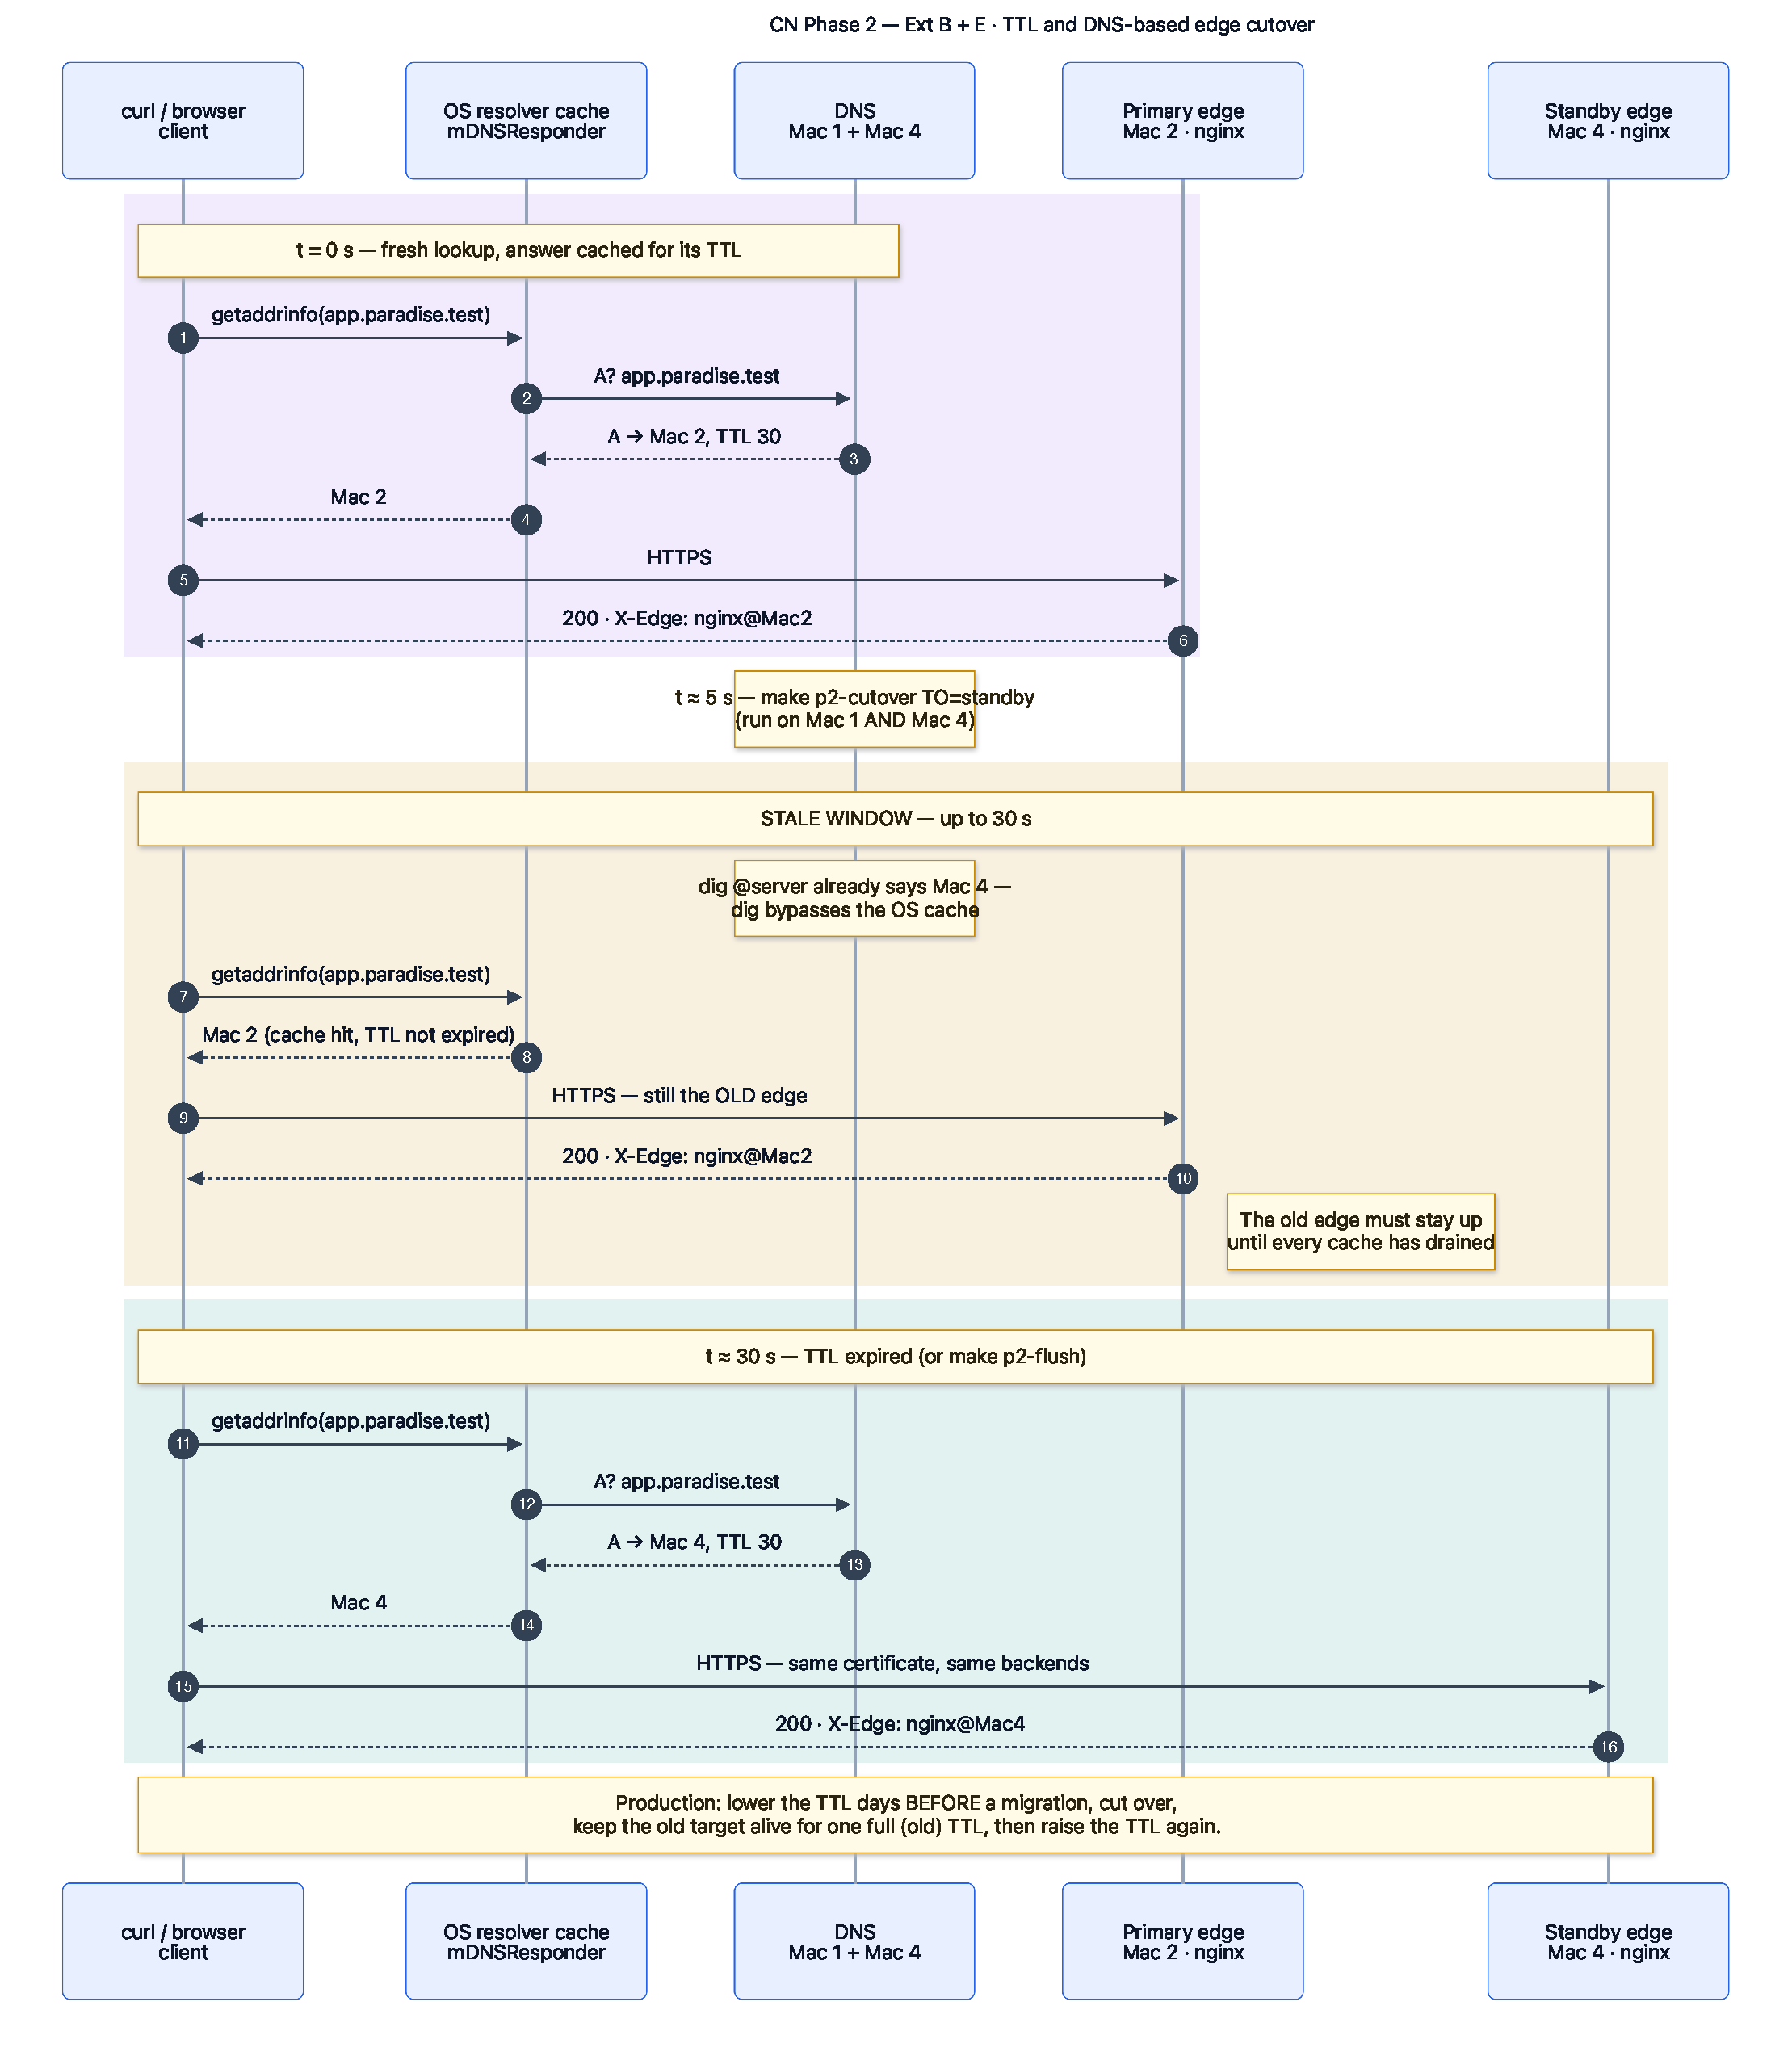
\includegraphics[height=0.62\textheight,keepaspectratio]{p2-ttl-cutover.pdf}
\caption{Ext~B/E sequence: the record changes on the server, but each client moves only when its cached answer expires or is flushed.}
\end{figure}

\begin{figure}[!htbp]
\centering
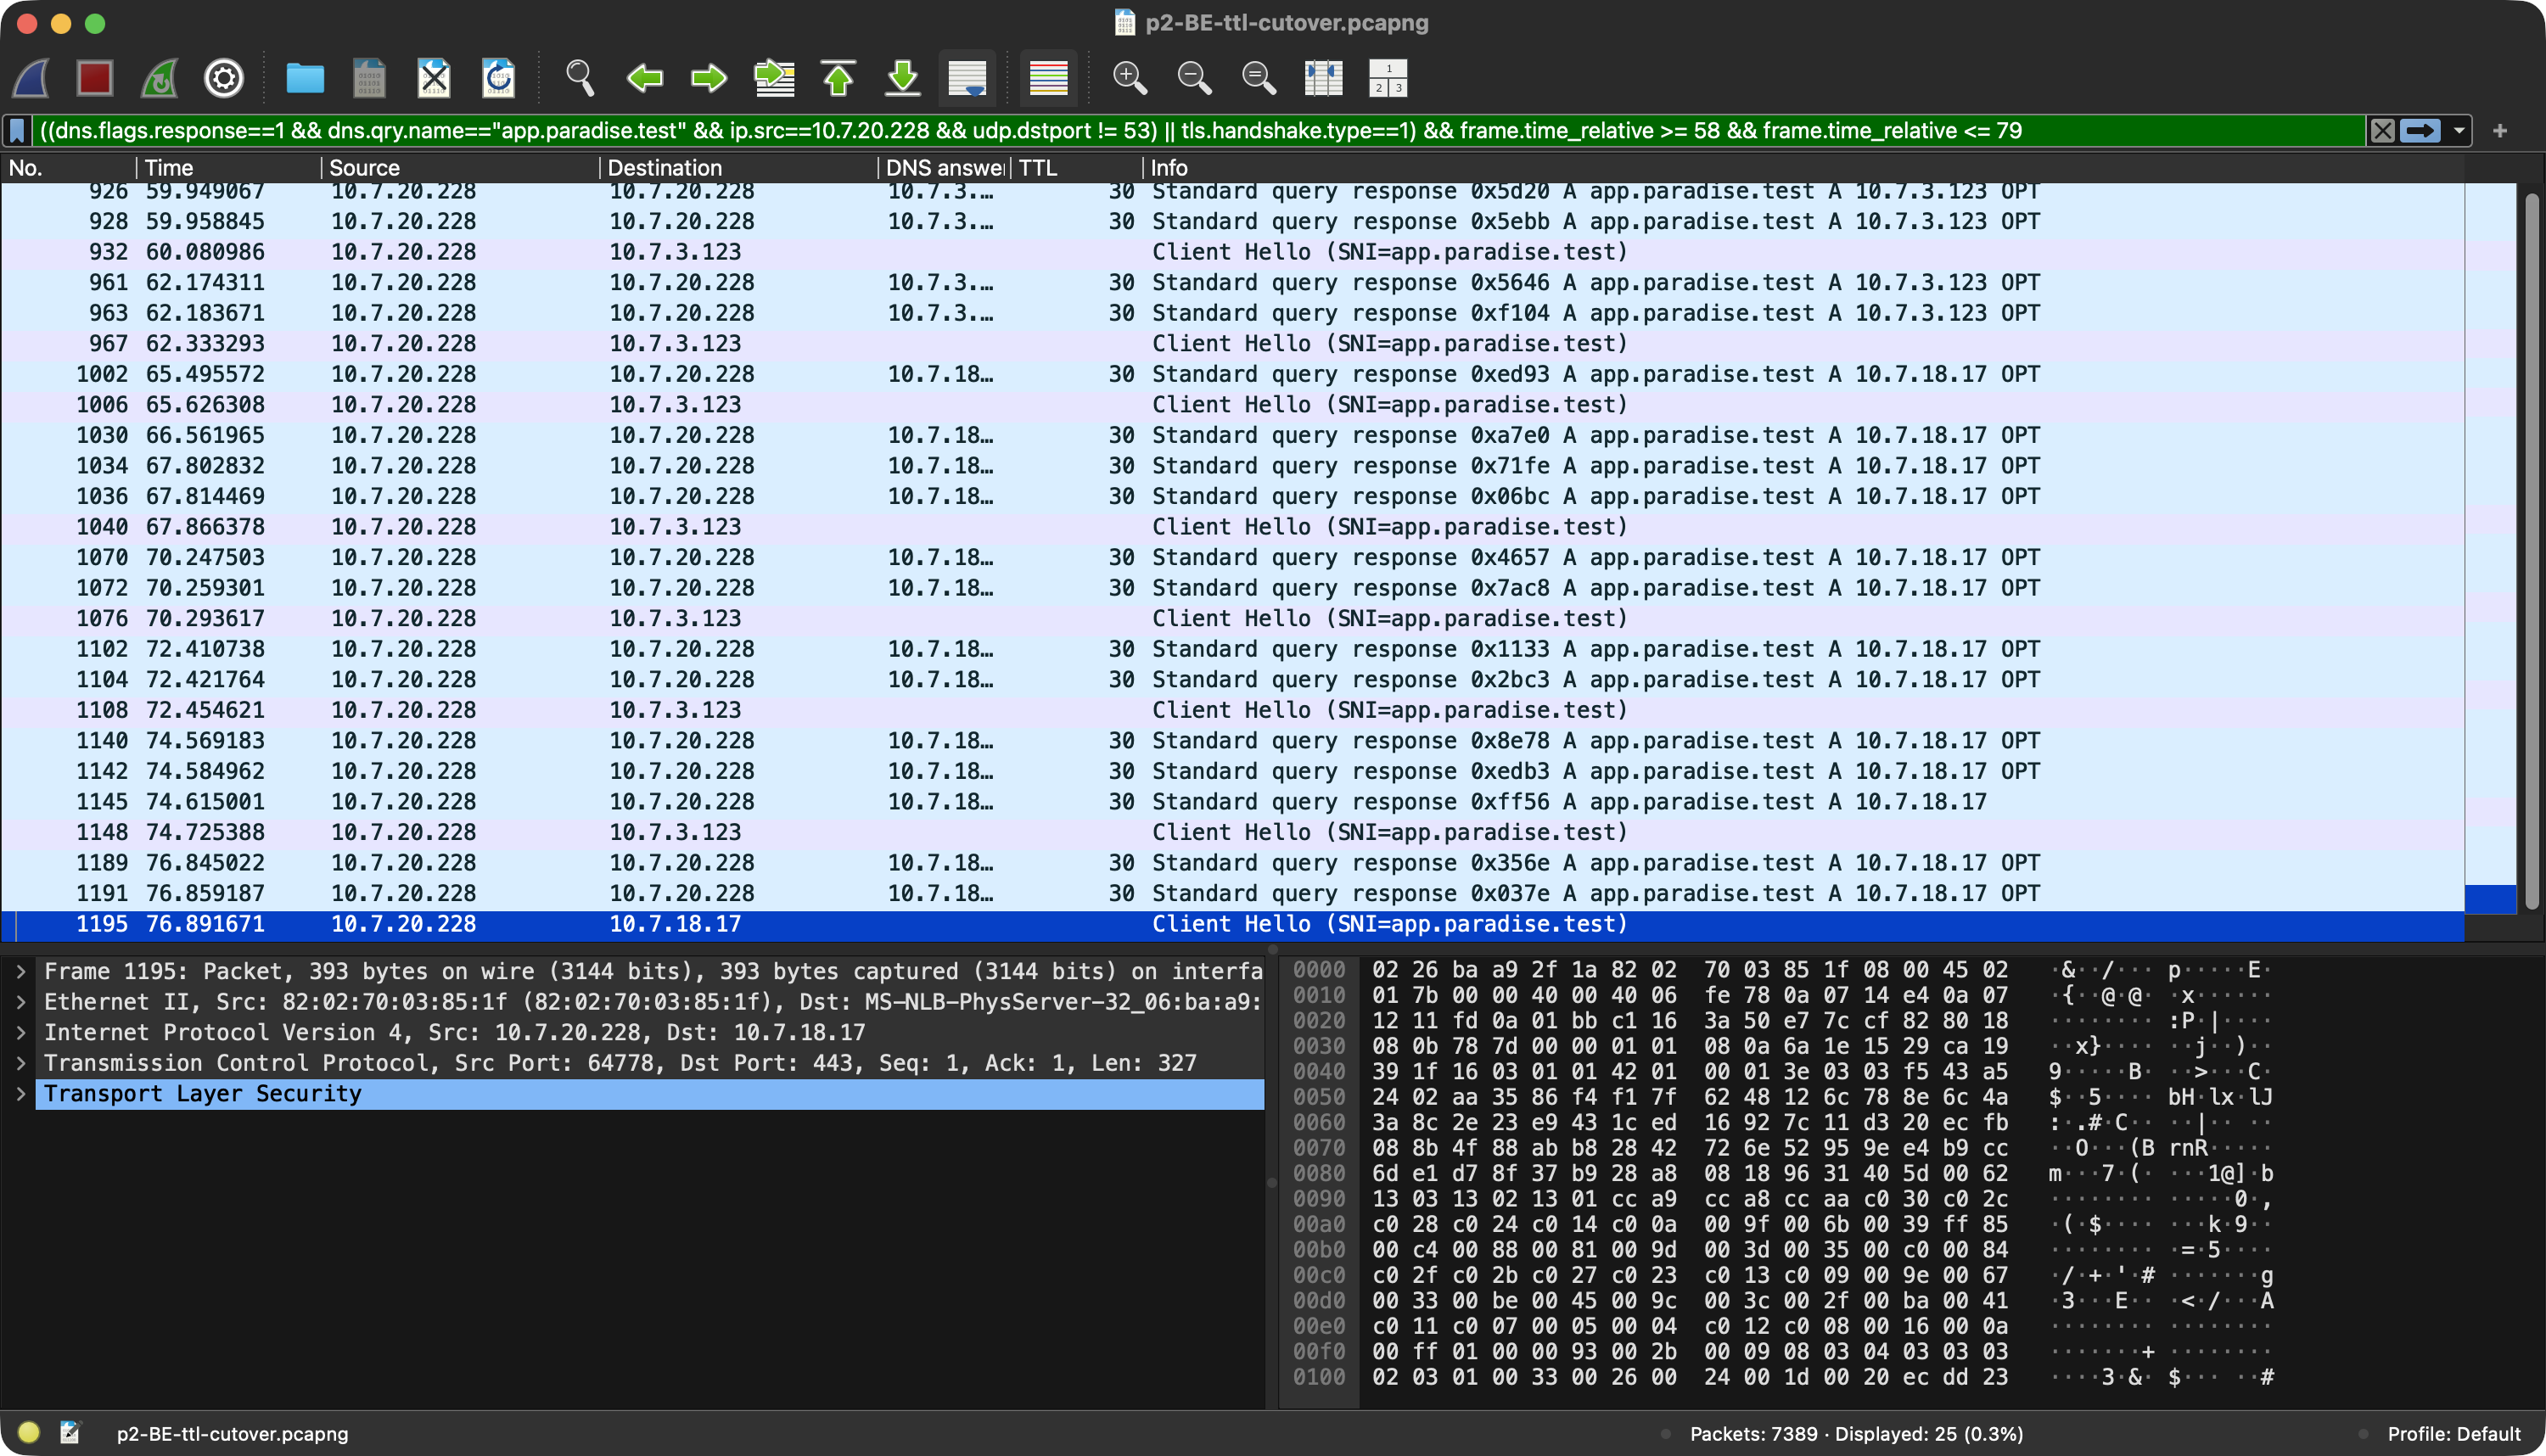
\includegraphics[width=0.9\textwidth]{W-B2-E1-dns-flips-then-clienthello-moves.png}
\caption{W-B2/E1: the DNS answer flips to 10.7.18.17, but ClientHellos keep going to 10.7.3.123 for another 11.4~s.}
\end{figure}

\subsection{Extension C --- Service isolation (pf)}
On Mac~3 and Mac~4 a pf anchor passes :3001/:3002 only from the two edges' IPs and
\texttt{block drop}s everything else. The spec says \emph{only Mac~2}; we also pass the standby edge
(Mac~4), because after an Ext~E cutover it must reach Backend~A. Clients are blocked either way.

\begin{table}[!htbp]
\centering
\caption{Ext~C probes.}
{\small
\begin{tabular}{@{}L{2.2cm}L{3.2cm}L{2.2cm}L{1.7cm}L{4.4cm}@{}}
\toprule
\textbf{Vantage point} & \textbf{Backend A :3001} & \textbf{Backend B :3002} & \textbf{Via edge} & \textbf{Evidence} \\
\midrule
Mac 1 (client) & \textbf{FILTERED} (3 s timeout, curl 28) & \textbf{FILTERED} & HTTP 200 & \texttt{C-probe-from-10.7.20.228}, \texttt{C1} \\
Mac 2 (edge) & \textbf{OPEN} (0 s) & \textbf{OPEN} (0 s) & HTTP 200 & \texttt{C-probe-from-10.7.3.123} \\
\bottomrule
\end{tabular}}
\end{table}

In \texttt{p2-C-isolation.pcapng}, Mac~1 sends 5 SYNs to \texttt{10.7.13.238:3001} at 0, 1, 2, 3 and
4~s (frames 1--5, all from ephemeral port 62233), then 5 to \texttt{10.7.18.17:3002}. There is no
SYN-ACK and no RST. A closed port answers with RST at once; a filtered port answers with nothing.

\begin{figure}[!htbp]
\centering
\resizebox{0.9\textwidth}{!}{\drawFiltered}
\caption{CLOSED versus FILTERED: two distinguishable transport-layer refusals.}
\end{figure}

\begin{figure}[!htbp]
\centering
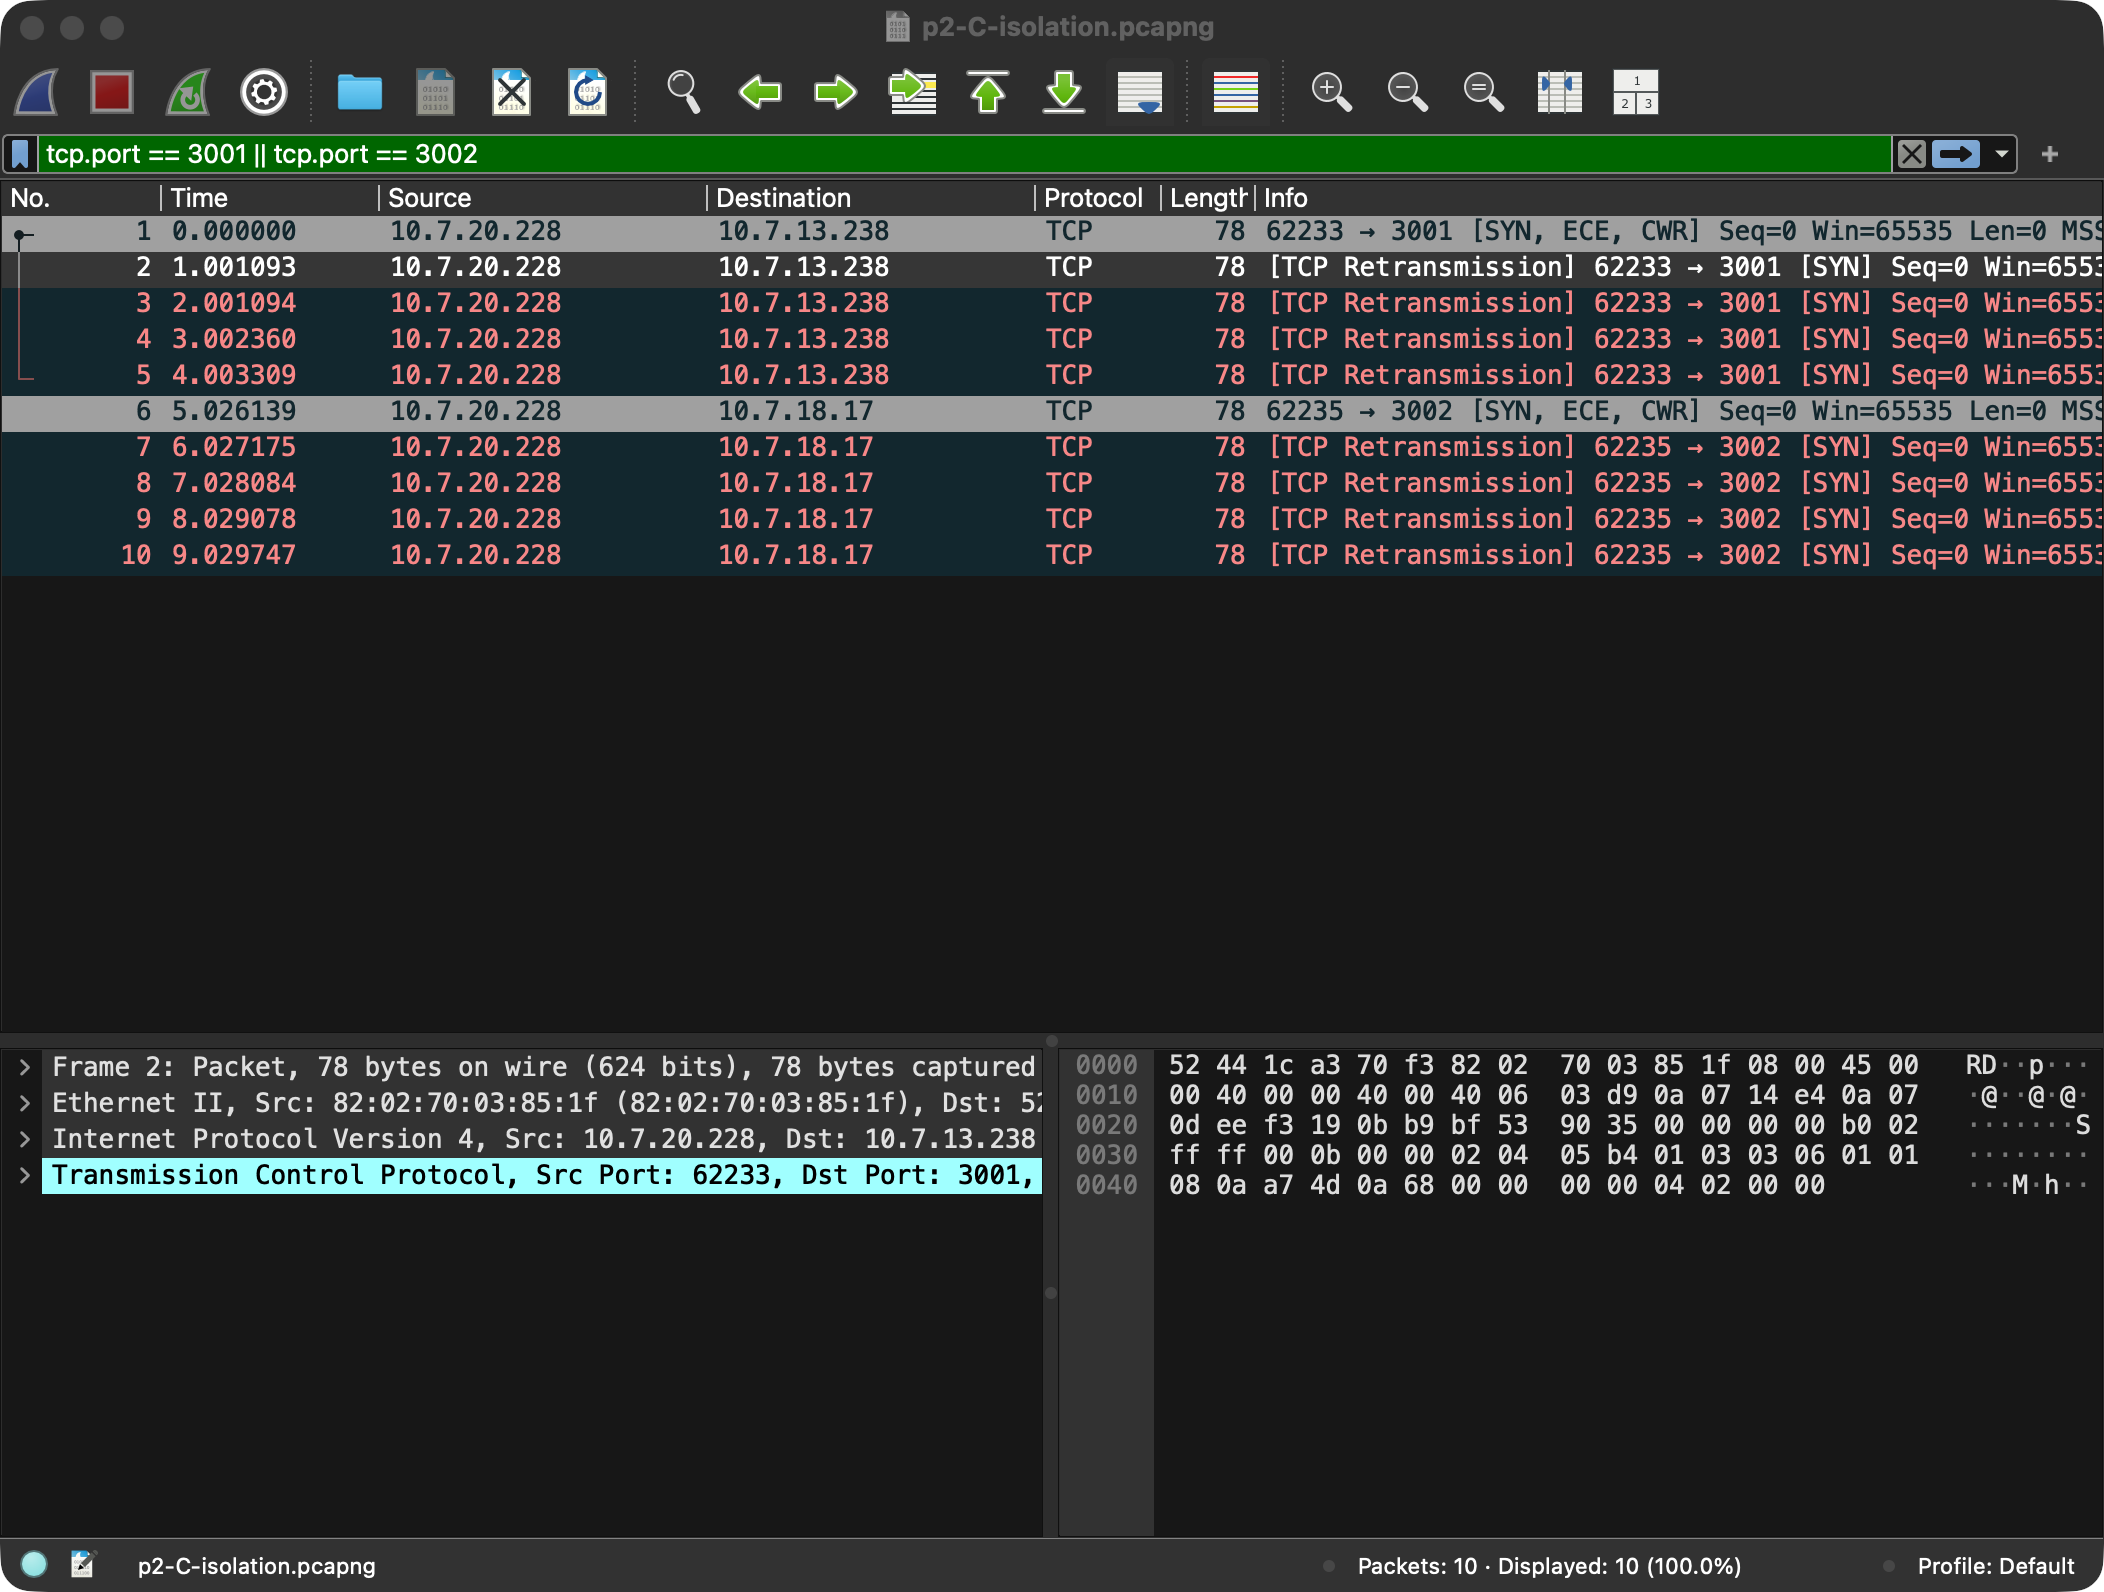
\includegraphics[width=0.8\textwidth]{W-C1-syn-retransmissions-filtered.png}
\caption{W-C1: SYN retransmissions to a filtered backend port, with no reply.}
\end{figure}

\subsection{Extension D --- High-availability failover}
Passive health checking: \texttt{max\_fails=1 fail\_timeout=10s} on both upstream servers, plus
\texttt{proxy\_next\_upstream error timeout http\_502 http\_503 http\_504} and
\texttt{proxy\_next\_upstream\_tries 2}. A failed attempt is retried on the other backend
\emph{inside the same client request}. \texttt{make p2-ha-demo} sent one request about every 0.7~s
for 100~s from Mac~1 while Tajuddin pressed Ctrl-C on Backend~A, then restarted it.

\begin{table}[!htbp]
\centering
\caption{HA failover run (\texttt{D-ha-demo-20261123-124350.txt}).}
{\small
\begin{tabular}{@{}L{6.4cm}L{7.8cm}@{}}
\toprule
\textbf{Measure} & \textbf{Value} \\
\midrule
Requests & \textbf{145} \\
Non-200 responses & \textbf{0} \\
Served by A / B & 46 / 99 \\
Longest B-only run & \textbf{37 consecutive responses}, 24 s $\to$ 49 s (A down) \\
Requests nginx retried off dead A & \textbf{9}: at 24, 25, 28, 35, 42, 43, 46, 47 s (and one isolated retry at 80 s) \\
A back in rotation & \textbf{50 s} \\
Checks & \textbf{6/6} \\
\bottomrule
\end{tabular}}
\end{table}

The 9 retries are how the client saw no errors: nginx tried A, got
\texttt{connect() failed (61: Connection refused)}, and replayed the request on B. Between retries
A was marked down for \texttt{fail\_timeout}; each time the 10~s ban expired, one request probed A
again, which is why the retries come in roughly 10~s steps. This clean run came \textbf{after}
fixing Incident~2; the same test before the fix gave six 502s.

\begin{figure}[!htbp]
\centering
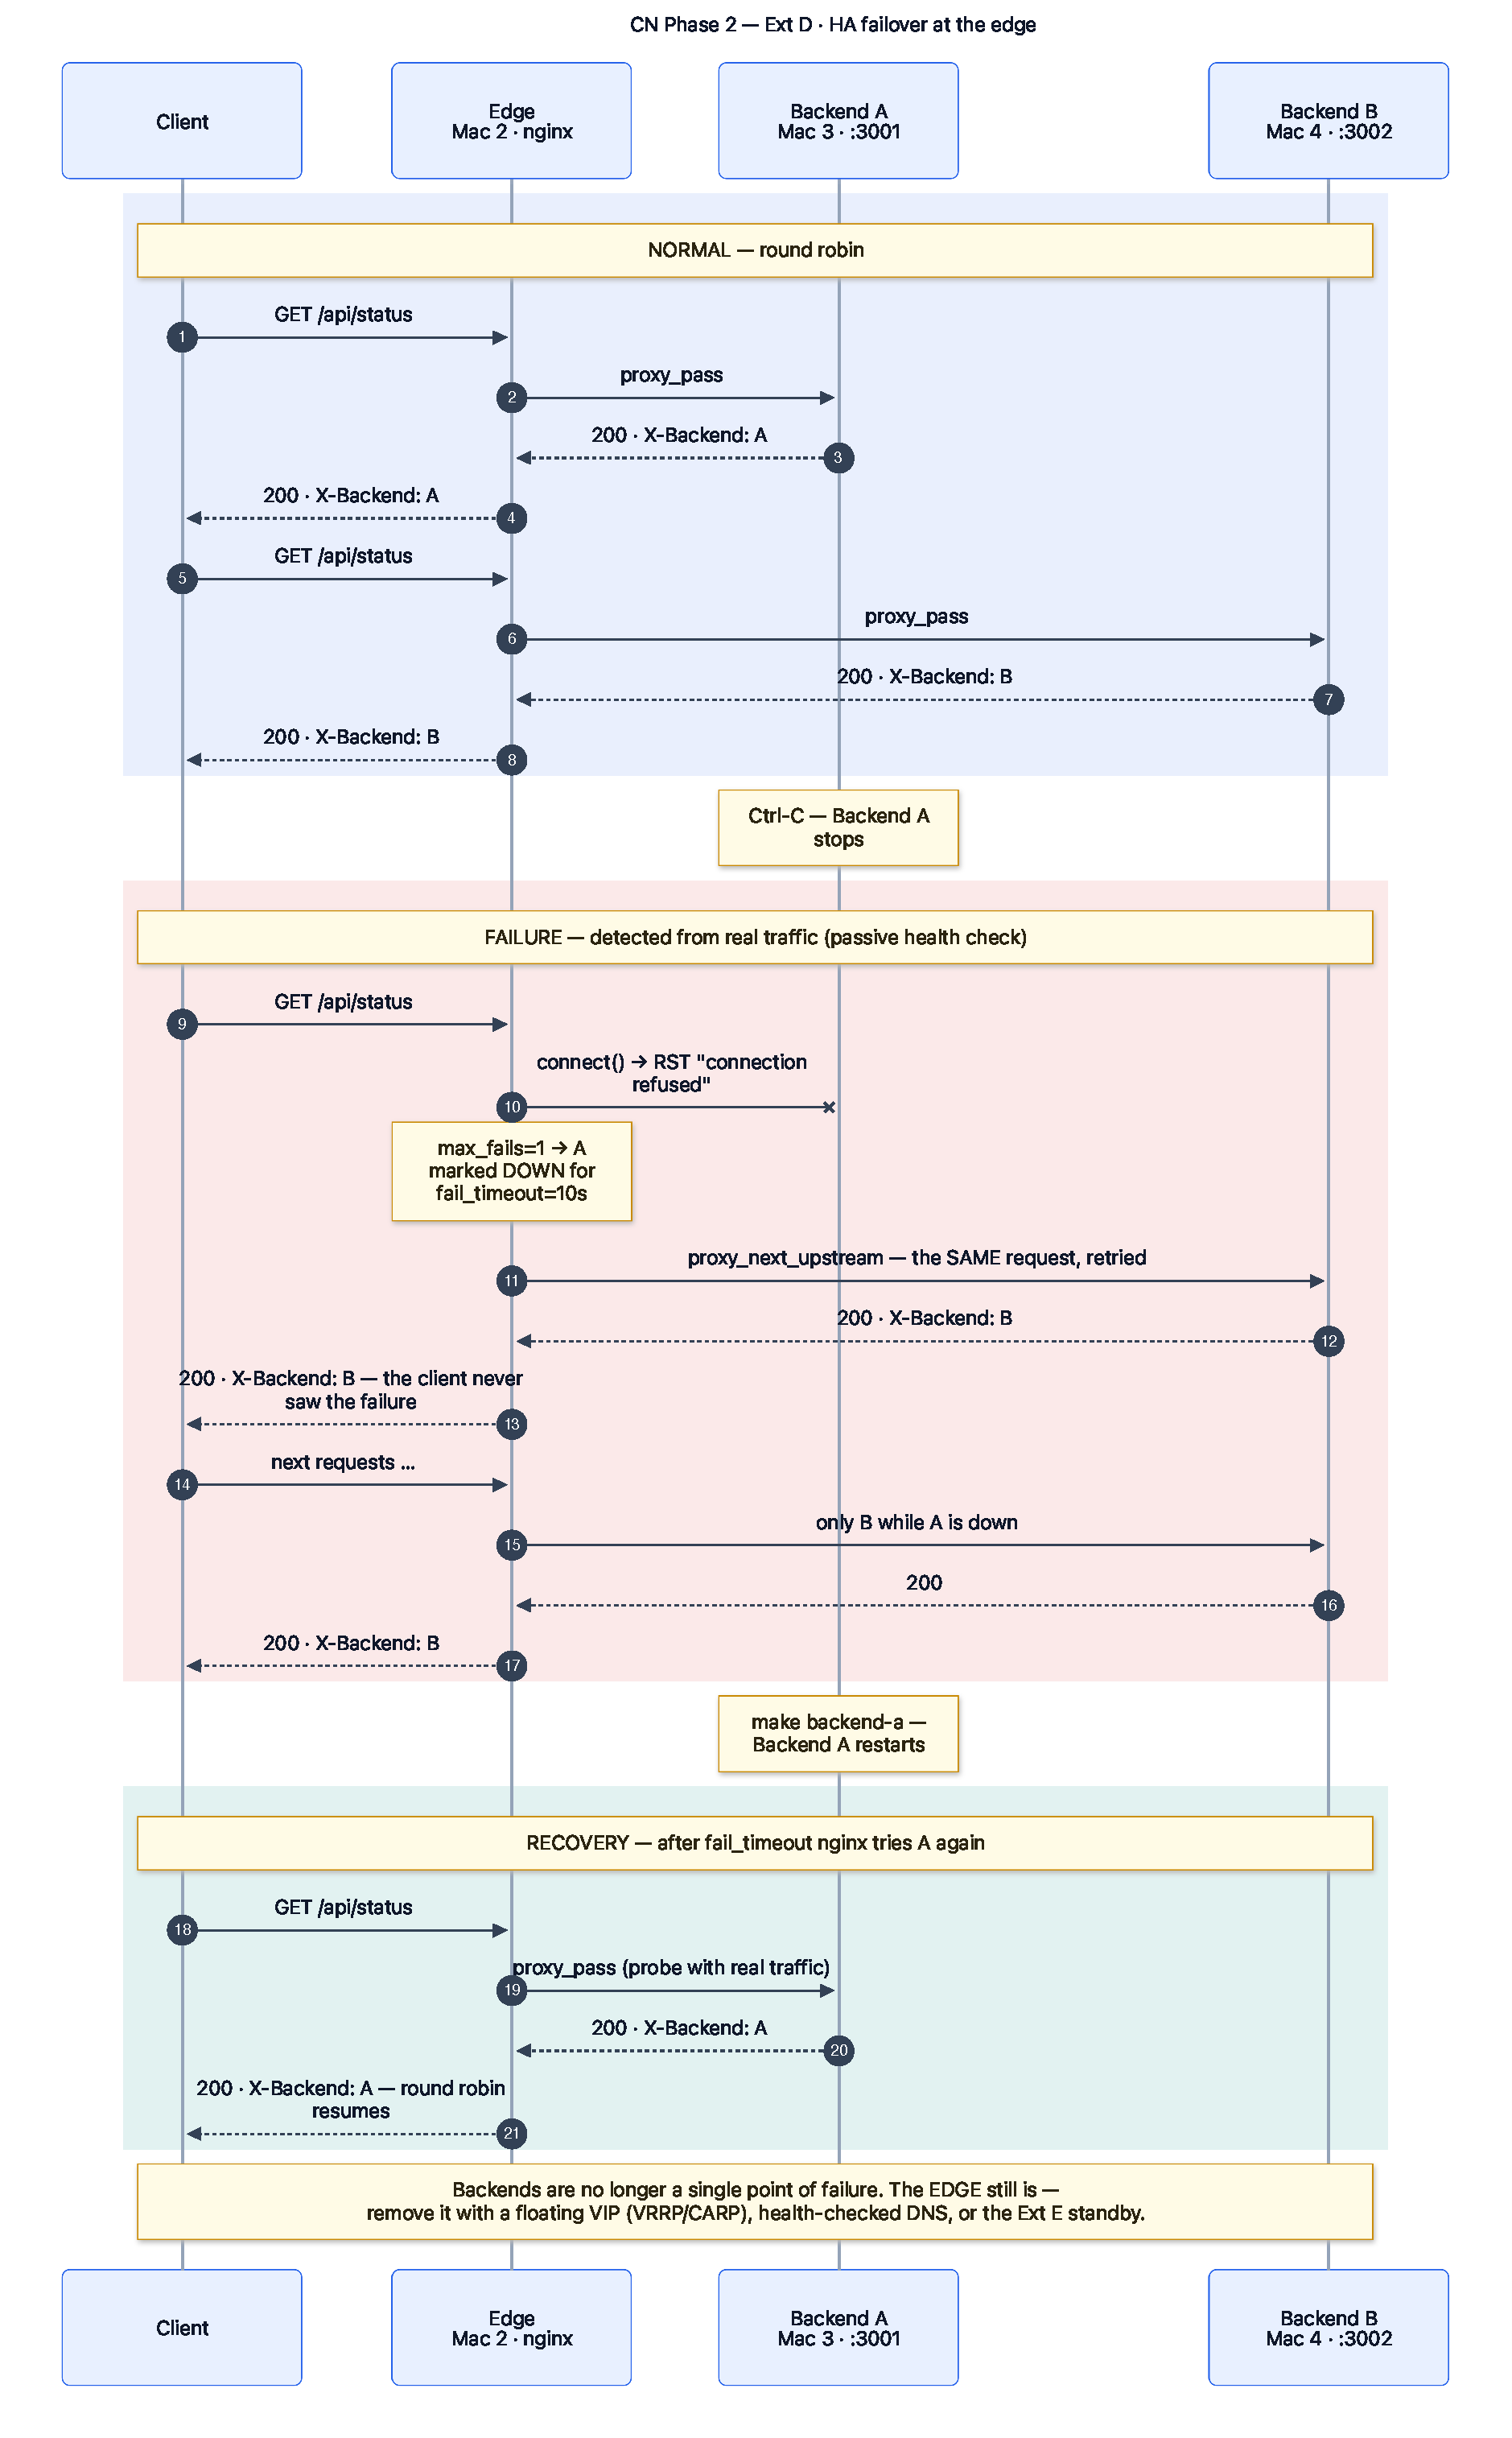
\includegraphics[height=0.62\textheight,keepaspectratio]{p2-ha-failover.pdf}
\caption{Ext~D sequence: a failed attempt on Backend~A is replayed on Backend~B within the same client request.}
\end{figure}

\subsection{Extension E --- Controlled edge migration}
Mac~4 runs a standby nginx with the same rendered config and the same certificate. Pinned with
\texttt{--resolve}, it completes a verified TLS 1.3 handshake without \texttt{-k} and identifies
itself as \texttt{X-Edge: nginx@10.7.18.17} (E1).

The cutover is the same run as Ext~B: changing the A records on both DNS servers moved traffic
from \texttt{nginx@10.7.3.123} to \texttt{nginx@10.7.18.17}. Clients that had cached the old answer
kept using the old edge for 9~s (sampled) or 11.4~s (on the wire). \textbf{No request failed in
either direction}, because the old edge stayed up until the cache had drained.

\begin{figure}[!htbp]
\centering
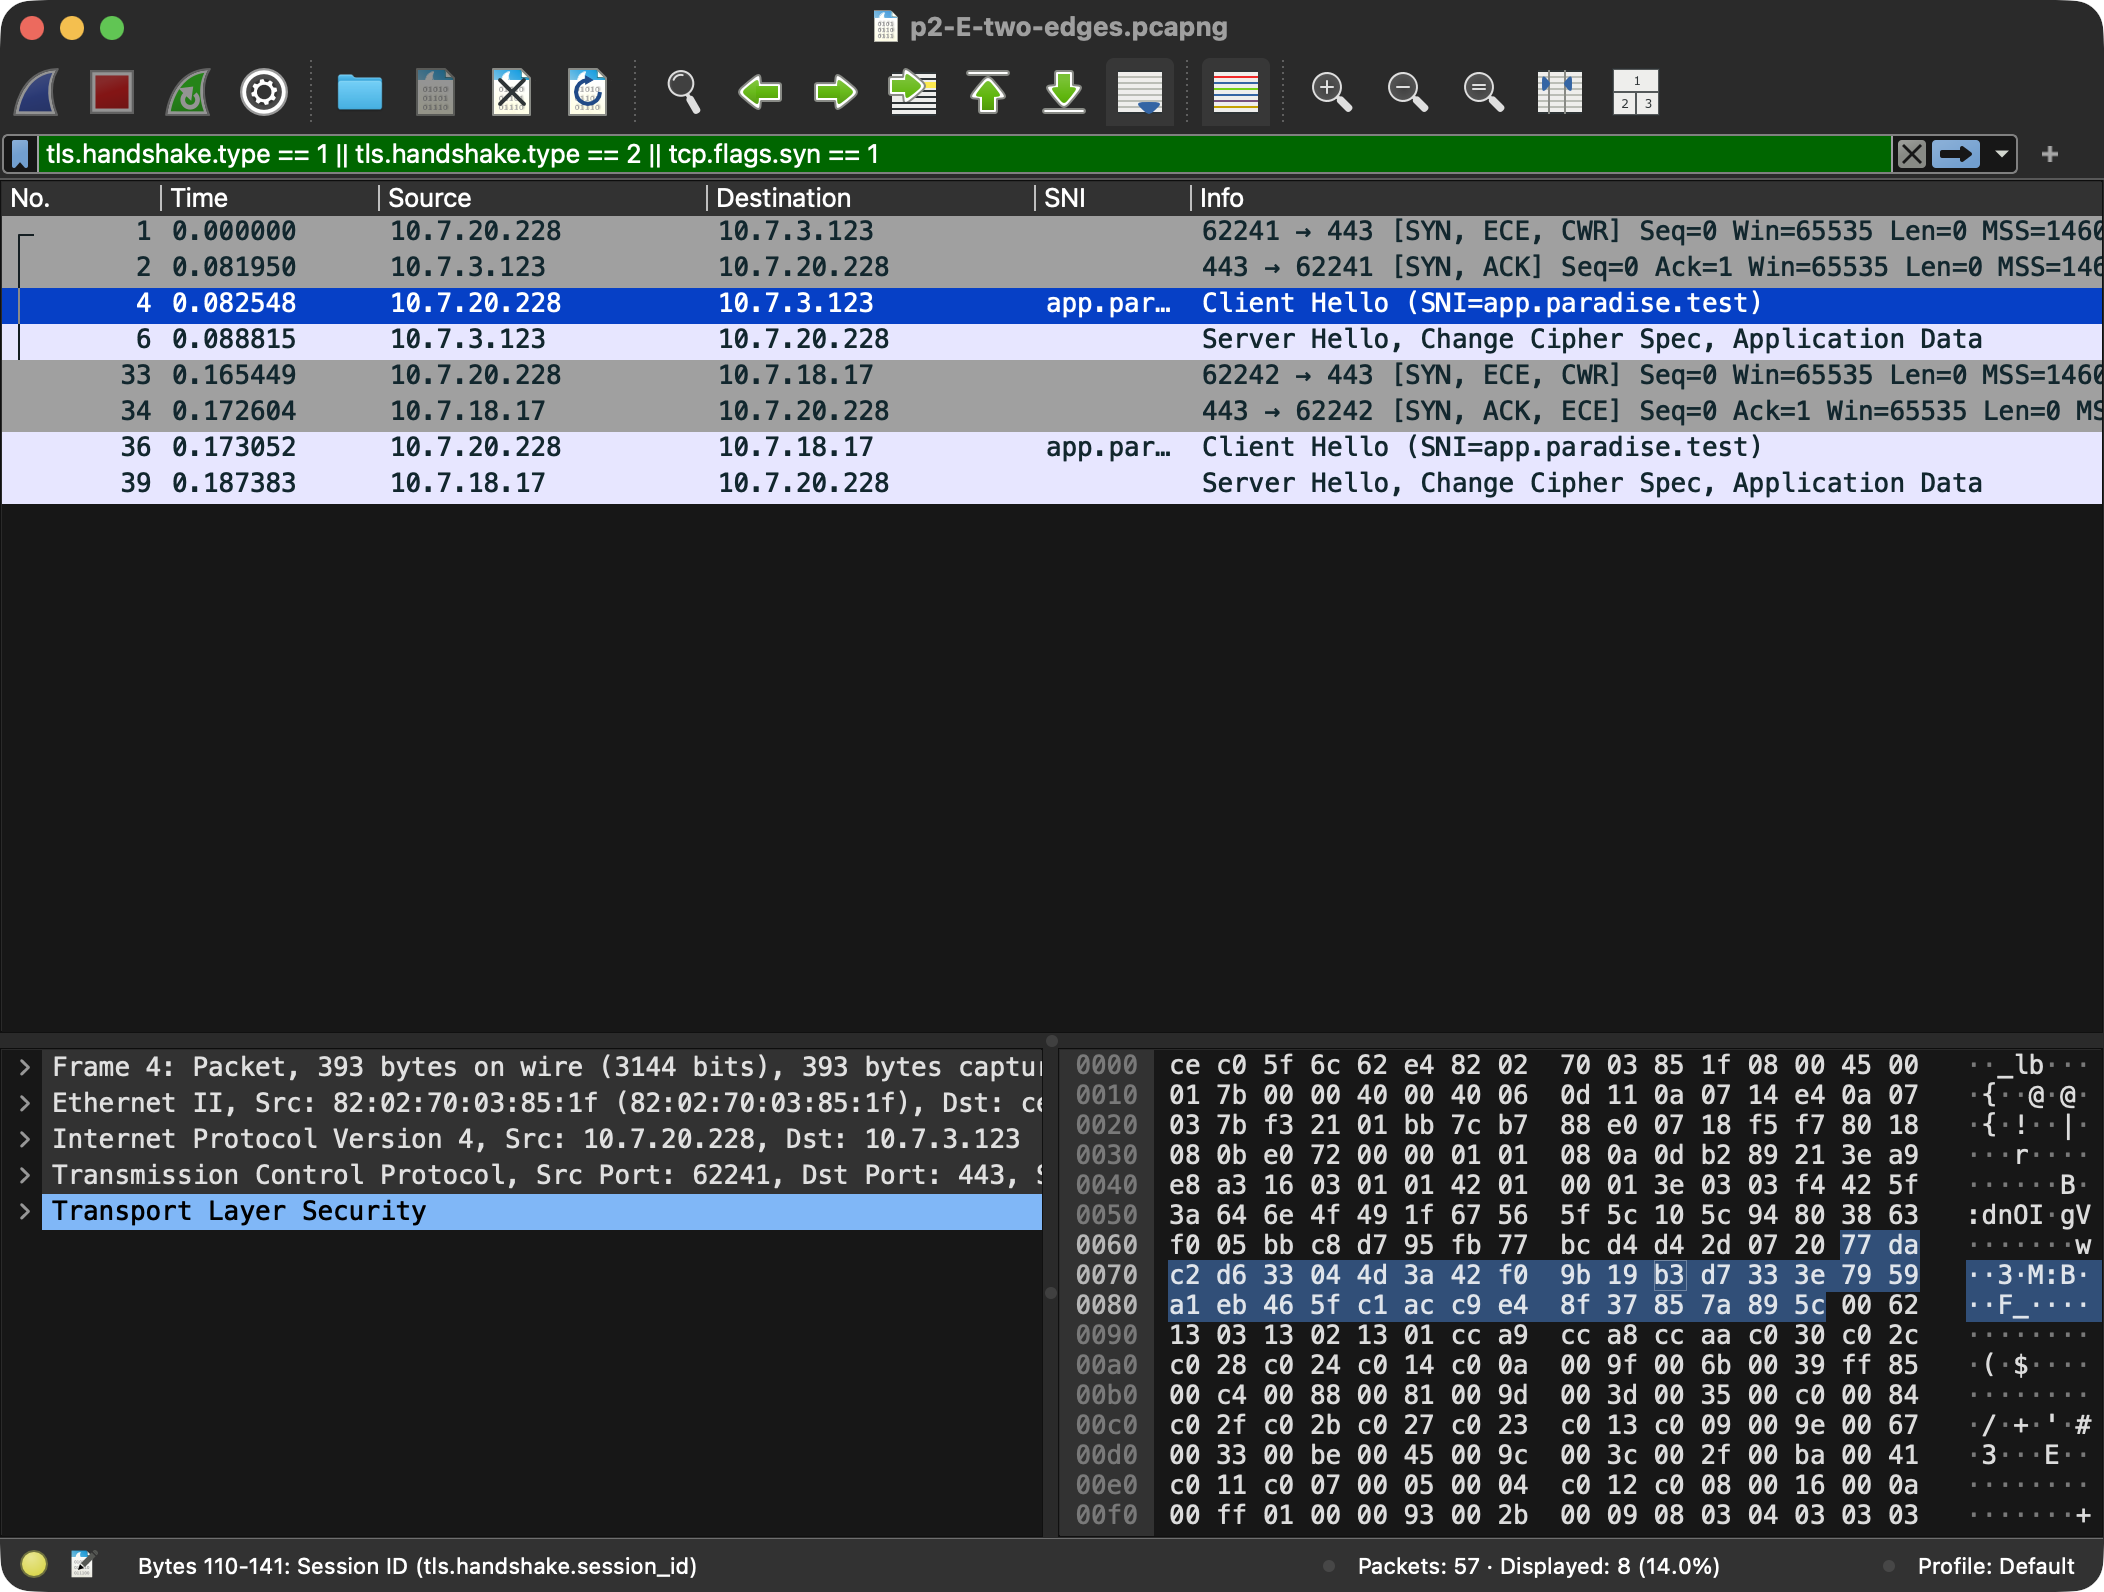
\includegraphics[width=0.8\textwidth]{W-E1-clienthello-both-edges.png}
\caption{W-E1: ClientHellos with the same SNI \texttt{app.paradise.test} to both edges.}
\end{figure}

\section{Real incidents found while running the demos}\label{sec:inc}
These were \textbf{not} injected. They happened during the live run, were diagnosed with the same
top-down method as Ext~F, and are kept in \texttt{evidence/phase2/F-troubleshooting/}.

\subsection{Incident 1 --- the primary edge vanished at the transport layer (12:27)}
\begin{table}[H]
\centering
\caption{Incident 1, layer by layer.}
{\small
\begin{tabular}{@{}L{2.0cm}L{6.0cm}L{6.2cm}@{}}
\toprule
\textbf{Layer} & \textbf{Check} & \textbf{Result} \\
\midrule
DNS & \texttt{dig app.paradise.test} & \ok\ 10.7.3.123 \\
IP & \texttt{ping 10.7.3.123} & \ok\ but $\sim$\textbf{800 ms RTT} (normal: 5--20 ms) \\
TCP & \texttt{nc -vz 10.7.3.123 443} and \texttt{:80} & \bad\ \textbf{timed out}: no SYN-ACK, no RST \\
Isolation & same test against standby 10.7.18.17:443 & \ok\ HTTP 200 \\
\bottomrule
\end{tabular}}
\end{table}
Verdict: transport layer, Mac~2 only, packets dropped (not refused). Cause: \textbf{Mac~2 had gone to
sleep}; its Wi-Fi could still answer ping slowly in power-save while nginx was frozen. Fix:
\texttt{caffeinate -dims} on every Mac. Lesson: ping proves layer~3 only, and \emph{timeout versus
refused} separates ``something is dropping packets'' from ``nothing is listening''.

\subsection{Incident 2 --- six 502s during HA failover: a keep-alive race (12:30)}
When Backend~A was stopped, requests \#22--\#36 included \textbf{six HTTP 502s}, although Backend~B
was running throughout.

\begin{table}[!htbp]
\centering
\caption{Incident 2 evidence.}
{\small
\begin{tabular}{@{}L{5.6cm}L{8.6cm}@{}}
\toprule
\textbf{Evidence} & \textbf{What it says} \\
\midrule
client: \texttt{upstream=10.7.18.17:3002, 10.7.13.238:3001, backend\_pool} & nginx tried \textbf{B first and B failed}, then A (dead), then had nothing left \\
client: \texttt{upstream=backend\_pool} & ``no live upstreams'': both peers marked down \\
Mac 2 error log, 12:30:54 & \texttt{upstream prematurely closed connection} on 10.7.18.17:3002 at \texttt{urt=0.092} s, so not a timeout \\
Mac 2 error log, 12:21:39 and 12:32:10 & the same failure on B and \texttt{Connection reset by peer} on A \textbf{in steady state}, invisible to clients \\
\bottomrule
\end{tabular}}
\end{table}

\begin{figure}[!htbp]
\centering
\resizebox{\textwidth}{!}{\drawKeepalive}
\caption{Root cause: two idle timers on the same TCP connection, in the wrong order.}
\end{figure}

After 5 idle seconds Node closed a pooled socket while an nginx worker sent the next request down
it. With both backends up, \texttt{proxy\_next\_upstream} retried on the other backend and nobody
noticed. With A dead, the retry went to A and failed; \texttt{max\_fails=1} then ejected B,
\textbf{the last healthy peer}, for 10~s, and every request in that window got 502. The fix orders
the timers so the side that reuses a connection gives it up before the side that closes it:

\par\noindent\begin{minipage}{\linewidth}
\begin{lstlisting}
# infra/mac2-edge/nginx/conf.d/site.conf.template, upstream backend_pool
keepalive_timeout 4s;

// services/backend/src/server.js
server.keepAliveTimeout = 65_000;
server.headersTimeout   = 66_000;   // must exceed keepAliveTimeout
\end{lstlisting}
\end{minipage}\par
Re-test: the identical demo gave \textbf{145 requests, 0 non-200}. Backend unit tests still pass
(8/8) and \texttt{make p2-test} passes (55/55).

\subsection{Incident 3 --- the campus gateway answers TCP for hosts that do not exist (13:04)}
While diagnosing the injected fault \texttt{dns-wrong-ip} (record $\to$ 10.255.255.1), ping failed but
\textbf{TCP :443 succeeded} for an address with no host behind it. Probing showed that :80 and :443
get a SYN-ACK from \emph{any} off-LAN address, :22 and ICMP get nothing, and TLS is then reset. The
SYN-ACK arrives with \textbf{IP TTL 63}, one less than our 64, so it comes from one hop away: the
gateway 10.7.0.1, a transparent proxy or firewall (\texttt{p2-F-middlebox.pcapng}). Lesson: a
passing TCP check proves that \emph{something} answered, not that the intended server did. The
diagnosis still named the correct layer because it reports the \textbf{first} failing layer.

\subsection{Incident 4 --- inconsistent DNS servers after a cutover (12:57--13:00)}
During the cut-back, the backup was twice left pointing at the standby while the primary pointed
at Mac~2: \texttt{TO=standby} was typed on Mac~4 instead of \texttt{TO=primary}.
\texttt{dig @10.7.20.228} returned 10.7.3.123 while \texttt{dig @10.7.18.17} returned 10.7.18.17.
Clients saw nothing because they ask the primary first, but had Mac~1 failed in that state every
client would have silently moved edge. We caught it by querying both servers directly; in
production, zone transfers keep secondaries consistent automatically.

\section{Troubleshooting findings (Extension F)}

\subsection{Method}
\texttt{make p2-diagnose} runs the layers in order and stops trusting the result at the
\textbf{first failure}; everything after it is either explained by it or untrustworthy.

\begin{figure}[!htbp]
\centering
\resizebox{0.96\textwidth}{!}{\drawDiagnose}
\caption{The top-down diagnosis ladder used by \texttt{diagnose.sh}.}
\end{figure}

\begin{table}[!htbp]
\centering
\caption{What each layer runs and what a failure means.}
{\small
\begin{tabular}{@{}L{0.4cm}L{2.0cm}L{6.0cm}L{5.8cm}@{}}
\toprule
\textbf{\#} & \textbf{Layer} & \textbf{Command} & \textbf{A failure means} \\
\midrule
0 & Local config & \texttt{networksetup -getdnsservers Wi-Fi}, \texttt{/etc/hosts} & the client asks the wrong server, or never asks \\
1 & DNS & \texttt{dig @primary}, \texttt{dig @backup}, \texttt{dig}, \texttt{dscacheutil} & no answer, or an answer that is neither edge \\
2 & Network & \texttt{ping <ip>} & host unreachable (caveats: Incidents 1 and 3) \\
3 & Transport & TCP connect to \texttt{:443} & \textbf{refused} = nothing listening; \textbf{timeout} = something drops \\
4 & TLS & \texttt{curl -v} without \texttt{-k} & certificate not trusted / wrong name / handshake failure \\
5 & HTTP & \texttt{curl -i} & 502/504 = edge up, backends not \\
\bottomrule
\end{tabular}}
\end{table}

\subsection{Injected faults}
\begin{table}[H]
\centering
\caption{Injected faults: per-layer results ( \ok\ pass, \bad\ fail, --- not reached).}
{\small
\begin{tabular}{@{}L{3.0cm}L{1.1cm}L{2.0cm}L{2.8cm}L{0.9cm}L{2.5cm}L{1.2cm}@{}}
\toprule
\textbf{Fault} & \textbf{On} & \textbf{0 Config} & \textbf{1 DNS} & \textbf{2 Ping} & \textbf{3 TCP} & \textbf{4 TLS} \\
\midrule
\texttt{dns-wrong-ip} & Mac 1 & \ok & \bad\ resolves to 10.255.255.1 & \bad & \ok* & \bad\ curl 35 \\
\texttt{edge-down} & Mac 2 & \ok & \ok\ 10.7.3.123 & \ok & \bad\ REFUSED (RST) & --- \\
\texttt{client-dns-wrong} & Mac 1 & \bad\ resolvers = 8.8.8.8 & \bad\ does not resolve & --- & --- & --- \\
\bottomrule
\end{tabular}}

\vspace{2pt}{\footnotesize * The campus gateway, not a real host (Incident 3).}
\end{table}

\begin{table}[!htbp]
\centering
\caption{Injected faults: verdict, fix and evidence.}
{\small
\begin{tabular}{@{}L{3.0cm}L{3.8cm}L{3.5cm}L{3.9cm}@{}}
\toprule
\textbf{Fault} & \textbf{Verdict} & \textbf{Fix} & \textbf{Evidence} \\
\midrule
\texttt{dns-wrong-ip} & \textbf{DNS (wrong record)} & \texttt{make p2-fault-undo} & \texttt{F-diagnose-...130423} \\
\texttt{edge-down} & \textbf{Transport (port closed)} & start nginx on Mac 2 & \texttt{F-diagnose-...130655}, F-2 \\
\texttt{client-dns-wrong} & \textbf{DNS (client resolver config)} & \texttt{make p2-client-dns} & \texttt{F-diagnose-...130829}, F-3 \\
\bottomrule
\end{tabular}}
\end{table}

Two earlier runs are also kept: \texttt{F-diagnose-...120030} is a genuine \textbf{TLS (trust)}
failure (every layer up to TCP passed, then curl 60, because Mac~1 did not yet trust the CA; fixed
with \texttt{make client-trust}, never \texttt{-k}), and \texttt{...120116} shows the same Mac healthy
46~s later.

\begin{figure}[!htbp]
\centering
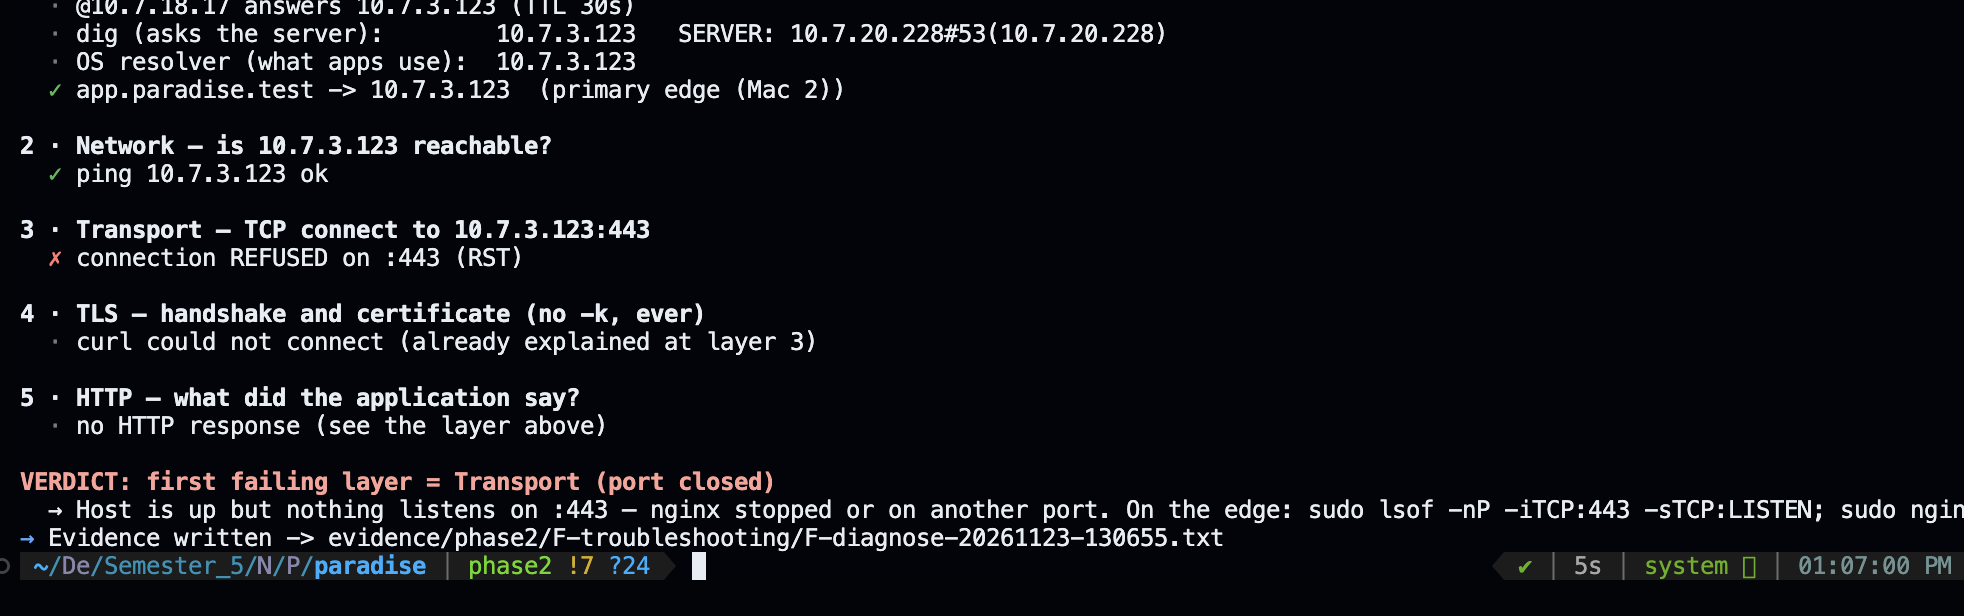
\includegraphics[width=\textwidth]{F-2-edge-down-verdict.png}
\caption{F-2: \texttt{p2-diagnose} with nginx stopped on Mac~2. DNS and ping pass; TCP is refused; verdict: transport.}
\end{figure}

\subsection{Faculty-injected fault (Review 2)}
To be filled in at the evaluation.\\[6pt]
\begin{tabular}{@{}ll@{}}
Fault: & \rule{9cm}{0.4pt} \\[8pt]
First failing layer: & \rule{9cm}{0.4pt} \\[8pt]
Command that showed it: & \rule{9cm}{0.4pt} \\[8pt]
Fix: & \rule{9cm}{0.4pt} \\[8pt]
Time to diagnose: & \rule{9cm}{0.4pt} \\
\end{tabular}

\subsection{What we take into the evaluation}
\begin{itemize}
  \item Always run the \textbf{standby edge} test at the transport step: it isolates ``this edge'' from ``the network'' in one command (Incident 1).
  \item Read \textbf{timeout versus refused} before anything else at the transport layer.
  \item When DNS is in question, query \textbf{both} servers directly; the default \texttt{dig} only shows the primary (Incident 4).
  \item Look in the edge's site error log, \texttt{paradise-error.log}, not the global \texttt{error.log}.
\end{itemize}

\section{Learning summary}

\paragraph{A --- Backup DNS.} A resolver list is a sequential fallback, not load balancing. The
client sends the query to the first server, waits about a second, and re-sends the \emph{same}
query (same transaction ID, \texttt{0x90b0}) to the next one. A primary outage therefore costs
every lookup roughly one second but never an answer. The backup must hold the records itself, or it
fails with the primary.

\paragraph{B --- TTL.} There are three answers to ``where does this name point'': the server's
(\texttt{dig}), the OS cache's (what applications use), and where TCP actually connects. They differ
for up to one TTL after a change; we measured 9~s sampled and 11.4~s on the wire with a 30~s TTL. A
flush removes the gap only on the machine that flushes, so a production migration lowers the TTL
well \emph{before} the cutover.

\paragraph{C --- Service isolation.} A firewall can refuse with a RST (CLOSED, immediate) or with
silence (FILTERED, SYN retransmissions). The rule matches by source IP: the same port is OPEN from
Mac~2 and FILTERED from Mac~1, which is AWS's ``inbound only from the load balancer's security
group''. A pf anchor plus a reference token made the rollback exact.

\paragraph{D --- HA failover.} Open-source nginx detects backend failure passively, from real
traffic, and \texttt{proxy\_next\_upstream} replays the request on the survivor: 9 retries out of
145 requests, 0 errors. The run that failed taught more: redundancy hides latent faults, and timer
ordering between proxy and backend (reuser $<$ closer) is a correctness requirement, not tuning.

\paragraph{E --- Edge migration.} DNS-based cutover is bounded by the TTL and is gradual: each
client moves when its own cache entry expires. The old edge must keep serving until the longest
TTL has drained, and both DNS servers must change together (Incident 4).

\paragraph{F --- Troubleshooting.} Diagnose top-down; the first failing layer is the verdict. Each
layer's check can mislead (ping on a sleeping host, TCP against a middlebox, one DNS server's view),
so each check is paired with a contrast: timeout versus refused, primary versus standby edge,
primary versus backup DNS.

\section{Remaining single point of failure}
\textbf{Edge selection.} The standby removes Mac~2 as a permanent SPOF, but failing over to it is a
\emph{manual} DNS change bounded by the TTL. Ways to remove it:
\begin{enumerate}
  \item a floating virtual IP (VRRP/keepalived, CARP): the standby claims the shared IP within about a second, with no DNS change;
  \item health-checked DNS failover (Route 53 failover records): DNS stops returning a dead edge automatically;
  \item anycast or a global load balancer in front of both edges.
\end{enumerate}

\textbf{Shared fate on Mac~4.} Backend~B, the backup DNS and the standby edge all run on Mac~4, on
different ports (:3002, :53, :80/:443). No single machine failure stops the service
(Mac~1 $\to$ Mac~2 $\to$ Mac~3 still works), but Mac~1 and Mac~4 failing together would leave no DNS
at all. Production spreads these across failure domains.

\section{Rollback}
Phase~2 keeps a rollback copy of everything it changes. After the evaluation, on each machine:
\par\noindent\begin{minipage}{\linewidth}
\begin{lstlisting}
make p2-rollback                  # everything Phase 2 changed on THIS machine
make p2-rollback WHAT=isolation   # Mac 3 / Mac 4: flush the pf anchor, release the token
make p2-status                    # confirm: no anchor, no standby nginx, resolvers restored
\end{lstlisting}
\end{minipage}\par
\texttt{p2-rollback} restores \texttt{dnsmasq.conf.pre-phase2}, the saved client resolver list, and
stops the standby nginx. The pf rules were applied only to the anchor, so nothing in
\texttt{/etc/pf.conf} needs restoring.

\section{Conclusion}
Phase~1 delivered a working private name, a trusted HTTPS edge, two identifiable load-balanced
backends, deterministic HTTP caching, and packet-level proof of DNS, TCP and TLS on four real
machines. Its failure demonstrations showed that each layer fails in its own, distinguishable way.

Phase~2 turned that working but fragile service into one that survives the loss of its primary
DNS server, a backend, and (by DNS cutover) its edge, with backend ports closed to everyone but the
edges. All six extensions were demonstrated live and the acceptance test passed 20/20 before and
after the demos. The most valuable result was not a passing demo but a failing one: the keep-alive
race showed that redundancy can hide latent faults until the moment it is needed. The remaining
single point of failure, manual edge selection, is named with three concrete ways to remove it.

\section{What is not in this report}
Machine-by-machine setup steps live in \texttt{docs/runbook.md}, \texttt{docs/phase2/README.md} and
the setup guide (\texttt{docs/index.html}); they are operational notes, not the academic
deliverable. Private keys, the CA key and the real \texttt{.env} are not committed.
Subnetting, NAT, DHCP, IPv6, routing and Ethernet framing (Weeks~7--12) are out of scope.

\clearpage
\appendix
\section{Phase 1 reference configuration}
Excerpts of the rendered files. Private keys are not included.

\subsection{dnsmasq (Mac 1, excerpt)}
\par\noindent\begin{minipage}{\linewidth}
\begin{lstlisting}
address=/app.paradise.test/10.7.8.155
address=/api.paradise.test/10.7.8.155
local-ttl=0
listen-address=0.0.0.0
bind-dynamic
no-resolv
server=1.1.1.1
domain-needed
bogus-priv
log-queries
\end{lstlisting}
\end{minipage}\par

\subsection{nginx upstream and proxy (Mac 2, excerpt)}
\needspace{8\baselineskip}
\begin{lstlisting}
upstream backend_pool {
    server 10.7.26.203:3001 max_fails=1 fail_timeout=10s;
    server 10.7.18.17:3002  max_fails=1 fail_timeout=10s;
    keepalive 16;
}
server {
    listen 443 ssl;  http2 on;
    server_name app.paradise.test api.paradise.test;
    ssl_protocols TLSv1.2 TLSv1.3;
    location / {
        proxy_pass http://backend_pool;
        proxy_http_version 1.1;
        proxy_set_header Connection "";
        proxy_next_upstream error timeout http_502 http_503 http_504;
        add_header X-Upstream-Addr $upstream_addr always;
        add_header X-Edge "nginx@10.7.8.155" always;
    }
}
\end{lstlisting}

\subsection{Backend contract}
\par\noindent\begin{minipage}{\linewidth}
\begin{lstlisting}
GET /api/status  ->  200
{"status":"ok","backend":"A"|"B","team":"paradise","host":...,"port":3001|3002}
X-Backend: A | B        X-Backend-Port: 3001 | 3002
Cache-Control: public, max-age=60        ETag: W/"..."   (weak)
\end{lstlisting}
\end{minipage}\par

\clearpage
\section{Phase 2 reference configuration}
Excerpts from \texttt{evidence/phase2/config-bundle/} (rendered on 23 November 2026). Private keys
are not included.

\subsection{dnsmasq, primary (Mac 1) and backup (Mac 4)}
Both files are identical; the backup has no \texttt{server=} line pointing at the primary.
\par\noindent\begin{minipage}{\linewidth}
\begin{lstlisting}
address=/app.paradise.test/10.7.3.123
address=/api.paradise.test/10.7.3.123
local-ttl=30
listen-address=0.0.0.0
bind-dynamic
no-resolv
server=1.1.1.1
domain-needed
bogus-priv
log-queries
\end{lstlisting}
\end{minipage}\par

\subsection{nginx upstream and failover (Mac 2; identical on the standby, Mac 4)}
\par\noindent\begin{minipage}{\linewidth}
\begin{lstlisting}
upstream backend_pool {
    server 10.7.13.238:3001 max_fails=1 fail_timeout=10s;
    server 10.7.18.17:3002 max_fails=1 fail_timeout=10s;
    keepalive 16;
    keepalive_timeout 4s;
}
location / {
    proxy_pass http://backend_pool;
    proxy_http_version 1.1;
    proxy_set_header Connection "";
    proxy_next_upstream error timeout http_502 http_503 http_504;
    proxy_next_upstream_tries 2;
    proxy_connect_timeout 2s;
}
\end{lstlisting}
\end{minipage}\par

\subsection{pf anchor \texttt{com.apple/250.ParadiseIsolation} (Mac 3; Mac 4 uses port 3002)}
\par\noindent\begin{minipage}{\linewidth}
\begin{lstlisting}
pass in quick on lo0 all
pass in quick proto tcp from { 10.7.3.123, 10.7.18.17 } to any port 3001 keep state
block drop in quick proto tcp from any to any port 3001
\end{lstlisting}
\end{minipage}\par

\subsection{Backend keep-alive (\texttt{services/backend/src/server.js})}
\par\noindent\begin{minipage}{\linewidth}
\begin{lstlisting}
server.keepAliveTimeout = 65_000;
server.headersTimeout   = 66_000;   // must exceed keepAliveTimeout
\end{lstlisting}
\end{minipage}\par

\section{Phase 2 evidence index}
\begin{table}[H]
\centering
\caption{Where each claim's evidence lives (\texttt{evidence/phase2/} and \texttt{evidence/captures/}).}
{\small
\begin{tabular}{@{}L{0.9cm}L{6.6cm}L{3.6cm}L{2.8cm}@{}}
\toprule
\textbf{Ext} & \textbf{Terminal output} & \textbf{Packets} & \textbf{Screenshots} \\
\midrule
A & \texttt{A-failover-demo}, \texttt{A1}, \texttt{A2}, \texttt{A3} & \texttt{p2-A-dns-failover} & W-A1, W-A2 \\
B & \texttt{B1}, \texttt{ttl-watch-...125354}, \texttt{ttl-watch-...125757} (flush) & \texttt{p2-B-ttl}, \texttt{p2-BE-ttl-cutover} & W-B1, W-B2-E1 \\
C & \texttt{C-probe-from-10.7.20.228}, \texttt{C-probe-from-10.7.3.123}, \texttt{C1} & \texttt{p2-C-isolation} & W-C1 \\
D & \texttt{D-ha-demo-20261123-124350}, \texttt{D1} & --- & --- \\
E & \texttt{E1}, the B watch files & \texttt{p2-E-two-edges}, \texttt{p2-BE-ttl-cutover} & W-E1, W-B2-E1 \\
F & 5 $\times$ \texttt{F-diagnose-*}, 3 $\times$ \texttt{F-incident*} & \texttt{p2-F-middlebox} & F-2, F-3 \\
all & \texttt{verify-phase2-...121147}, \texttt{verify-phase2-...130949}, config bundle & & \\
\bottomrule
\end{tabular}}
\end{table}
\end{document}
